\documentclass[10pt,a4paper]{article}

% ============================================================================
%  TP3 Optimización 2026 2C — "Diseño de Supermercados" (CarroMenos)
%  Martínez Folica, Nazareno · Naón, Pedro
%
%  Compilar con dos pasadas de pdflatex (índice y referencias cruzadas).
%  Las figuras se leen de ../resultados/graficos/: correr antes los scripts.
%
%  Nota de maquetación: todas las tablas y figuras usan [H] (paquete float)
%  para que aparezcan exactamente donde están declaradas.
% ============================================================================

\usepackage[utf8]{inputenc}
\usepackage[T1]{fontenc}
\usepackage{lmodern}
\usepackage[a4paper,margin=2.2cm,headheight=14pt]{geometry}
\usepackage{graphicx}
\usepackage{booktabs}
\usepackage{array}
\usepackage{tabularx}
\usepackage{float}
\usepackage[table]{xcolor}
\usepackage{amsmath}
\usepackage{amssymb}
\usepackage{enumitem}
\usepackage{caption}
\captionsetup{font=small,skip=4pt}
\usepackage{subcaption}
\usepackage{needspace}
\usepackage{fancyhdr}
\usepackage{titlesec}
\usepackage{tikz}
\usetikzlibrary{arrows.meta,calc,positioning}
\usepackage[colorlinks=true,linkcolor=accentlink,citecolor=accentlink,urlcolor=accentlink,linktoc=all]{hyperref}
\usepackage{xurl}

% ---------- paleta ----------------------------------------------------------
\definecolor{limita}{HTML}{2A78D6}
\definecolor{accent}{HTML}{1F4E79}
\definecolor{accentlink}{HTML}{1F5C99}
\definecolor{centroA}{HTML}{2A78D6}
\definecolor{centroC}{HTML}{EB6834}
\definecolor{centroD}{HTML}{1BAF7A}
\definecolor{planta}{HTML}{1B8A4A}

% ---------- tipografía de títulos -------------------------------------------
\titleformat{\section}{\normalfont\Large\bfseries\color{accent}}{\thesection}{0.6em}{}
\titleformat{\subsection}{\normalfont\large\bfseries\color{accent}}{\thesubsection}{0.6em}{}
\titleformat{\subsubsection}{\normalfont\bfseries\color{accent}}{\thesubsubsection}{0.6em}{}
\titlespacing*{\section}{0pt}{1.1em}{0.55em}
\titlespacing*{\subsection}{0pt}{0.9em}{0.4em}

\pagestyle{fancy}
\fancyhf{}
\renewcommand{\headrulewidth}{0.4pt}
\fancyhead[L]{\small Optimización 2026 2C — Diseño de Supermercados (CarroMenos)}
\fancyhead[R]{\small Martínez Folica, N. · Naón, P.}
\fancyfoot[C]{\small\thepage}

\setlength{\parskip}{0.25em}
\setlist[itemize]{topsep=0.2em, itemsep=0.05em}
\setlist[enumerate]{topsep=0.2em, itemsep=0.05em}

\newcommand{\cuello}[1]{\textbf{\textcolor{limita}{#1}}}
\newcommand{\cita}[1]{\emph{``#1''}}

\renewcommand{\contentsname}{Índice}
\renewcommand{\figurename}{Figura}
\renewcommand{\tablename}{Tabla}

\begin{document}

% ============================================================================
\begin{titlepage}
\begin{center}
\vspace*{1.2cm}
{\large UCA}\\[2pt]
{\large Facultad de Ingeniería y Ciencias Agrarias}\\[1.4cm]

{\large Optimización — 2026, 2\textdegree{} Cuatrimestre}\\[0.3cm]
{\large Trabajo Práctico N.\textdegree{} 3}\\[1.8cm]

\rule{0.85\linewidth}{0.6pt}\\[0.5cm]
{\Huge\bfseries\color{accent} Diseño de Supermercados}\\[0.5cm]
{\Large Localización de centros de distribución para CarroMenos\\
con programación lineal entera mixta e indicadores ambientales}\\[0.5cm]
\rule{0.85\linewidth}{0.6pt}\\[2.2cm]

\begin{tabular}{c}
{\large\bfseries Integrantes} \\[0.4cm]
{\large Martínez Folica, Nazareno} \\[0.15cm]
{\large Naón, Pedro}
\end{tabular}

\vfill

{\large 23 de octubre de 2026}
\end{center}
\end{titlepage}

\pagenumbering{roman}
\tableofcontents
\newpage
\pagenumbering{arabic}

% ============================================================================
\section*{Introducción}
\addcontentsline{toc}{section}{Introducción}

CarroMenos es una cadena de supermercados que hoy delega la gestión de su
cadena de suministro en Goyito, una empresa de logística \cita{que cuenta con
clientes con mayor prioridad y envergadura}. Para asegurar el abastecimiento,
la cadena evalúa instalar un \textbf{centro de distribución propio}
\cite{consigna}. El problema tiene tres niveles: \textbf{siete plantas} que
fabrican cinco productos (fideos, arroz, leche, gaseosas y galletitas), un
conjunto de \textbf{cuatro localizaciones candidatas} para los centros (A, B, C
y D) y \textbf{diez supermercados} que demandan en conjunto
\textbf{51.850 pallets por mes}. El tramo de las plantas a los centros lo
cubren camiones tercerizados a una tarifa por kilómetro; el de los centros a
los supermercados, camiones propios, que consumen gasoil y requieren
conductores.

Las decisiones son dos y están encadenadas: \textbf{qué centros abrir} y
\textbf{cuántos pallets de cada producto recorren cada tramo de la red}. El
criterio es el costo total mensual —apertura, operación de los centros,
transporte, conductores y, si corresponde, un gerente de coordinación—, y la
consigna pide además cuantificar \textbf{el consumo de combustible y las
emisiones de CO$_2$} de cada configuración.

La consigna contiene dos listas que conviene no confundir. La primera, el
\emph{informe esperable por la cátedra}, define la estructura de este
documento: el modelo (Sección~\ref{sec:modelo}), el análisis de sensibilidad
(Sección~\ref{sec:sensibilidad}), la representación gráfica de los flujos
(Sección~\ref{sec:grafica}) y las librerías utilizadas
(Sección~\ref{sec:librerias}). La segunda contiene las \textbf{cinco
preguntas} sobre el caso, que se responden en la Sección~\ref{sec:preguntas}.

\paragraph{Naturaleza del problema.} Aunque la consigna habla de un
\emph{modelo de programación lineal}, abrir o no un centro es una decisión de
sí o no con costo fijo, y el gerente se contrata según una regla lógica. El
problema es un \textbf{problema de localización de instalaciones}
(\emph{facility location}) \cite{scipbook}: un modelo de \textbf{programación
lineal entera mixta}, con variables binarias para los centros y continuas para
los flujos, que combina la estructura de red de transbordo \cite{catedra-redes}
con las restricciones lógicas de la programación entera \cite{catedra-mip}.
Esa naturaleza condiciona el análisis de sensibilidad: con variables enteras
no hay análisis post-óptimo directo, y la Sección~\ref{sec:sensibilidad}
explica cómo se resolvió.

% ============================================================================
\section{Modelo de programación lineal}
\label{sec:modelo}

\subsection{Supuestos más importantes}
\label{sec:supuestos}

La consigna es precisa en los datos de los centros, las tarifas y la demanda,
pero deja abiertos varios puntos sin los cuales el modelo no puede escribirse:
las distancias, la capacidad de un camión, el costo de los conductores, la
forma de medir las emisiones. Cada supuesto se adoptó con una justificación y,
cuando admite otra lectura razonable, se convirtió en un parámetro del modelo
para evaluar su incidencia (Sección~\ref{sec:tests}). Los valores que no
provee la consigna se obtuvieron de fuentes externas, citadas en la
bibliografía.

\paragraph{S1 — Las distancias se miden por calle.} La consigna pide
\cita{utilizar los datos del mapa}. El mapa de la cátedra se descargó con las
coordenadas exactas de sus 21 puntos y las distancias se calcularon por la red
de calles con el motor de ruteo OSRM \cite{osrm} sobre la cartografía de
OpenStreetMap \cite{osm}. Un camión no viaja en línea recta: la distancia por
calle resultó, en la mediana, \textbf{1,27 veces} la distancia en línea recta,
con un rango de 1,14 a 1,51 entre los percentiles 10 y 90. La matriz además
\textbf{no es simétrica} —hasta 7,7\,km de diferencia entre ida y vuelta, por
calles de una mano y accesos a autopistas—, y el modelo usa la ida y la vuelta
reales. La alternativa, línea recta por el factor de ruta, se evalúa como
test.

\paragraph{S2 — El centro principal es uno solo: A o B.} La consigna establece
que la empresa \cita{debe elegir su centro principal para lo cual cuenta con
dos opciones}. \emph{Elegir} entre \emph{dos opciones} es excluyente, de modo
que se impone que se abra exactamente uno de los dos. La lectura alternativa,
que permite abrir ambos, se evalúa como test.

\paragraph{S3 — La condición sobre C y D se cumple siempre.} La consigna
habilita los centros C y D \cita{sólo si la demanda de productos supera a la
capacidad del centro A o B}. La demanda total (51.850 pallets) supera la
capacidad de A (40.000) y la de B (35.000): la condición es siempre verdadera
y no genera restricción alguna. Por la misma razón, \textbf{ningún centro
alcanza por sí solo} y toda solución abre al menos dos.

\paragraph{S4 — El gerente se contrata con tres o más centros.} La exigencia
de un gerente \cita{al abrir tres centros de distribución al mismo tiempo} se
interpreta como tres o más: coordinar cuatro centros no es más sencillo que
coordinar tres.

\paragraph{S5 — Un camión transporta 26 pallets y los viajes son proporcionales
a los pallets.} Sin la capacidad del camión no es posible pasar de pallets a
viajes, ni de viajes a kilómetros. Se adoptan \textbf{26 pallets}, la carga
máxima de un semirremolque estándar con pallets de 1,00\,×\,1,20\,m no
remontables \cite{dsv}, y el mismo camión en ambos tramos, coherente con el
único rendimiento que informa la consigna. En cada tramo, la cantidad de
viajes es pallets\,/\,26, con un único destino por viaje y retorno vacío. La
construcción de rutas con varias paradas —un problema de ruteo de vehículos,
emparentado con el agente viajante \cite{catedra-redes}— queda fuera del
alcance y se declara como limitación: el modelo mide el transporte con la
precisión de un modelo de localización, no con la de un plan de rutas.

\paragraph{S6 — Kilómetros físicos de ida y vuelta; tarifa sobre la ida.}
El camión propio consume gasoil en la ida y en la vuelta vacía, y lo mismo
ocurre con las emisiones de cualquier camión. La tarifa del tercerizado, en
cambio, se interpreta como un precio por kilómetro \emph{de recorrido} del
servicio, que ya incorpora el retorno del transportista. La lectura
alternativa, que aplica la tarifa sobre ida y vuelta, se evalúa como test.

\paragraph{S7 — Costo de los conductores.} La consigna pide \cita{agregar el
costo mensual de los conductores} sin informarlo. Se adopta un costo de
\textbf{\$\,1.600.000 por conductor y por mes}: el básico del conductor de
primera categoría del convenio colectivo de camioneros (CCT 40/89) vigente en
octubre de 2026, \$\,1.126.149,40 \cite{cct}, más el aguinaldo proporcional y
las contribuciones del empleador (31,4\,\% en total). Cada conductor puede
recorrer como máximo \textbf{7.700\,km por mes}: los 22 días de trabajo que
garantiza el convenio por los 350\,km diarios que el mismo convenio toma como
referencia para los viajes. La cantidad de conductores es una variable entera
del modelo.

\paragraph{S8 — Indicadores ambientales.} Los litros de gasoil se obtienen
como kilómetros físicos dividido el rendimiento de 4\,km/l que informa la
consigna, y las emisiones como litros por \textbf{2,68\,kg de CO$_2$ por
litro}, el factor por defecto del IPCC para el gasoil \cite{ipcc} con una
densidad de 0,84\,kg/l. El camión tercerizado se supone igual al propio, a
falta de otro dato.

\paragraph{S9 — El funcional minimiza el costo; lo ambiental se cuantifica y
se explora.} La consigna pide minimizar el costo total \cita{considerando,
además, indicadores ambientales}. El \emph{además} indica un criterio
secundario: el funcional minimiza el costo en pesos, cada solución informa sus
litros y su CO$_2$, y el compromiso entre ambos se mide con una frontera
costo–emisiones (Sección~\ref{sec:frontera}). Incorporar un precio del carbono
dentro del funcional se evalúa como test.

\paragraph{S10 — Supuestos menores.} Los costos de apertura se toman como
costos mensuales, igual que el sueldo del gerente (la consigna no indica
período; el test~G muestra que la decisión no depende de este punto). La
capacidad de un centro limita los pallets que opera en el mes. Las plantas no
tienen límite de producción, de modo que fideos y leche, que tienen dos plantas
cada uno, se abastecen de la que resulte más conveniente. Los flujos se
modelan por producto y como variables continuas: con 51.850 pallets por mes, el
redondeo es irrelevante. Rigen los supuestos generales de la programación
lineal —proporcionalidad, aditividad y certidumbre—, salvo la divisibilidad de
las decisiones de apertura y de conductores.

\begin{table}[H]
\centering\small
\caption{Supuestos del modelo y alternativas evaluadas.}
\label{tab:supuestos}
\begin{tabularx}{\linewidth}{@{}llXl@{}}
\toprule
\textbf{ID} & \textbf{Supuesto} & \textbf{Lectura adoptada} & \textbf{Alternativa (test)} \\
\midrule
S1 & Distancias              & Por calle (OSRM)                          & Línea recta × 1,27 (A) \\
S2 & Centro principal        & Exactamente uno de A y B                  & Al menos uno (B) \\
S3 & Condición de C y D      & Siempre cumplida                          & --- \\
S4 & Gerente                 & Con tres o más centros                    & --- \\
S5 & Camión y viajes         & 26 pallets, viajes proporcionales         & 20 a 30 pallets (C) \\
S6 & Ida y vuelta            & Física ida y vuelta; tarifa sobre la ida  & Tarifa ida y vuelta (D) \\
S7 & Conductores             & \$\,1,6\,M por mes; 7.700\,km por mes     & ±30\,\%; 6.000 a 12.000\,km (E) \\
S8 & Emisiones               & 4\,km/l; 2,68\,kg CO$_2$/l                & --- \\
S9 & Criterio ambiental      & Se cuantifica y se explora                & Precio del carbono (F) \\
S10 & Apertura               & Costo mensual                             & ×0,05 a ×2 (G) \\
\bottomrule
\end{tabularx}
\end{table}

\subsection{Variables de decisión}
\label{sec:variables}

Sean $K$ los cinco productos, $P$ las siete plantas (con $P_k$ las que fabrican
el producto $k$), $J = \{A, B, C, D\}$ los centros e $I = \{S1, \dots, S10\}$
los supermercados. El modelo decide:

\[
\begin{array}{lll}
y_j \in \{0,1\}       & j \in J              & \text{1 si se abre el centro } j \\[2pt]
g \in \{0,1\}         &                      & \text{1 si se contrata el gerente de coordinación} \\[2pt]
x_{pj} \geq 0         & p \in P,\ j \in J    & \text{pallets por mes de la planta } p \text{ al centro } j \\[2pt]
z_{jik} \geq 0        & j \in J,\ i \in I,\ k \in K & \text{pallets por mes del producto } k \text{ del centro } j \text{ al súper } i \\[2pt]
n \in \mathbb{Z}_{\geq 0} &                  & \text{conductores propios}
\end{array}
\]

Son \textbf{234 variables}: 5 binarias, una entera general y 228 continuas
(28 flujos de planta a centro y 200 de centro a supermercado), sujetas a 277
restricciones. El producto de cada flujo $x_{pj}$ queda determinado por la
planta de origen. Para la pregunta~e) se agrega la variable continua
$\mathit{exc} \geq 0$, los kilómetros que exceden el tope pactado con el
sindicato, y para la pregunta~c) una binaria $u_k$ por producto, que vale 1 si
el producto lo transporta Goyito.

\subsection{Función objetivo}
\label{sec:objetivo}

El objetivo es minimizar el costo total mensual:
\[
\begin{aligned}
\text{Min } Z \;=\; & \sum_{j} F_j\, y_j \;+\; G\, g \;+\; \sum_{j} c_j \sum_{i,k} z_{jik}
&& \text{apertura, gerente y operación} \\
+\; & \sum_{p,j} \frac{T\, d_{pj}}{Q}\, x_{pj}
&& \text{tercerizado, planta} \to \text{centro} \\
+\; & \sum_{j,i} \frac{C_K\,(d_{ji}+d_{ij})}{Q} \sum_k z_{jik}
&& \text{combustible, centro} \to \text{súper} \\
+\; & W\, n
&& \text{conductores}
\end{aligned}
\]

Cada término de transporte es un costo por pallet: el costo de un viaje por la
fracción de camión que ocupa un pallet ($1/Q$). En el tramo tercerizado se
paga la tarifa $T$ sobre la distancia de ida $d_{pj}$; en el propio, el
combustible $C_K = 1.300\,/\,4 = \$\,325$ por kilómetro físico sobre la ida y
la vuelta. Las preguntas~d) y~e) modifican este funcional sin cambiar su
estructura (Sección~\ref{sec:preguntas}).

Los indicadores ambientales se calculan sobre las mismas variables:
\[
\text{km} = \sum_{p,j} \frac{d_{pj}+d_{jp}}{Q}\, x_{pj} + \sum_{j,i} \frac{d_{ji}+d_{ij}}{Q}\sum_k z_{jik},
\qquad
\text{litros} = \frac{\text{km}}{4},
\qquad
\text{CO}_2 = 2{,}68 \cdot \text{litros}.
\]

\subsection{Parámetros}
\label{sec:parametros}

\begin{table}[H]
\centering\small
\caption{Centros de distribución candidatos \cite{consigna}.}
\label{tab:centros}
\begin{tabular}{lrrr}
\toprule
\textbf{Centro} & \textbf{Capacidad [pallets/mes]} $\mathit{cap}_j$ & \textbf{Apertura [\$/mes]} $F_j$ & \textbf{Operación [\$/pallet]} $c_j$ \\
\midrule
A & 40.000 & 3.000.000 & 10 \\
B & 35.000 & 2.500.000 & 12 \\
C & 15.000 & 1.200.000 & 5 \\
D & 10.000 & 900.000 & 8 \\
\bottomrule
\end{tabular}
\end{table}

\begin{table}[H]
\centering\small
\caption{Demanda mensual promedio por producto y supermercado [pallets] \cite{consigna}.}
\label{tab:demanda}
\setlength{\tabcolsep}{4.5pt}
\begin{tabular}{lrrrrrrrrrrr}
\toprule
\textbf{Producto} & \textbf{S1} & \textbf{S2} & \textbf{S3} & \textbf{S4} & \textbf{S5} & \textbf{S6} & \textbf{S7} & \textbf{S8} & \textbf{S9} & \textbf{S10} & \textbf{Total} \\
\midrule
Fideos     & 2000 & 1900 & 1800 & 2100 & 2500 & 3000 & 1200 & 1700 & 2100 & 2000 & 20.300 \\
Arroz      & 1000 &  900 &  800 & 1200 &  500 &  400 &  850 & 1200 &  800 &  900 &  8.550 \\
Leche      &  750 &  800 &  900 & 1100 & 1200 &  950 & 1000 & 1100 &  950 & 1200 &  9.950 \\
Gaseosas   &  300 &  400 &  500 &  540 &  340 &  500 &  450 &  400 &  520 &  600 &  4.550 \\
Galletitas &  800 &  900 &  850 &  750 &  950 & 1000 &  950 &  850 &  800 &  650 &  8.500 \\
\midrule
\textbf{Total} & 4850 & 4900 & 4850 & 5690 & 5490 & 5850 & 4450 & 5250 & 5170 & 5350 & \textbf{51.850} \\
\bottomrule
\end{tabular}
\end{table}

\begin{table}[H]
\centering\small
\caption{Parámetros escalares. Los marcados con $\ast$ no figuran en la consigna.}
\label{tab:escalares}
\begin{tabularx}{\linewidth}{@{}lrlX@{}}
\toprule
\textbf{Parámetro} & \textbf{Valor} & \textbf{Unidad} & \textbf{Fuente} \\
\midrule
$T$ tarifa del tercerizado          & 500       & \$/km de ida        & Consigna \\
$C_K$ combustible del camión propio & 325       & \$/km físico        & Consigna: \$\,1.300/l, 4\,km/l \\
$G$ gerente de coordinación          & 2.000.000 & \$/mes              & Consigna \\
$Q$ pallets por camión$^\ast$        & 26        & pallets/viaje       & DSV \cite{dsv} \\
$W$ costo de un conductor$^\ast$     & 1.600.000 & \$/mes              & CCT 40/89 \cite{cct} + aguinaldo y cargas \\
$K_{\max}$ km por conductor$^\ast$   & 7.700     & km/mes              & CCT 40/89: 22 días × 350\,km \\
$\varphi$ factor de emisión$^\ast$   & 2,68      & kg CO$_2$/l         & IPCC 2006 \cite{ipcc} \\
$d$ distancias$^\ast$                & 21 × 21   & km                  & OSRM \cite{osrm} sobre el mapa de la consigna \\
\bottomrule
\end{tabularx}
\end{table}

Las distancias determinan los coeficientes por pallet de cada arco de la red.
En la mediana, un pallet viaja 28\,km de la planta al centro, a un costo de
\$\,531 con el tercerizado, y 22\,km del centro al supermercado, a \$\,597 de
combustible, frente a los \$\,5 a \$\,12 por pallet que cuesta operar un
centro.

\subsection{Restricciones}
\label{sec:restricciones}

\begin{table}[H]
\centering\small
\caption{Restricciones del modelo y su origen en la consigna.}
\label{tab:restricciones}
\renewcommand{\arraystretch}{1.25}
\begin{tabularx}{\linewidth}{@{}lp{5.4cm}X@{}}
\toprule
\textbf{ID} & \textbf{Restricción} & \textbf{Origen} \\
\midrule
R1 & $\sum_j z_{jik} = \mathit{dem}_{ik}\quad \forall\, i,k$ & \cita{Abastecer la demanda}: cada supermercado recibe exactamente su demanda de cada producto (50 restricciones). \\
R2 & $\sum_{p \in P_k} x_{pj} = \sum_i z_{jik}\quad \forall\, j,k$ & Conservación del flujo: lo que sale de un centro entró desde una planta de ese producto (20). \\
R3 & $\sum_{i,k} z_{jik} \leq \mathit{cap}_j\, y_j\quad \forall\, j$ & Capacidad mensual de cada centro. Además liga el flujo a la apertura: un centro cerrado no opera. \\
R4 & $z_{jik} \leq \mathit{dem}_{ik}\, y_j\quad \forall\, j,i,k$ & Formulación reforzada \cite{scipbook}: redundante en la solución entera, ajusta la relajación lineal. \\
R5 & $y_A + y_B = 1$ & \cita{Debe elegir su centro principal […] dos opciones} (S2). \\
R6 & $g \geq \sum_j y_j - 2$ & \cita{Al abrir tres centros […] un gerente de coordinación} (S4). \\
R7 & $K_{\max}\, n \geq \text{km}_{\text{propios}}$ & Los conductores tienen que alcanzar para los kilómetros de la flota propia (S7). \\
\bottomrule
\end{tabularx}
\end{table}

La restricción R7 es la que vincula la flota propia con el costo de personal:
cada conductor habilita 7.700\,km por mes, y el modelo elige el número entero
de conductores necesario. Las preguntas~d) y~e) agregan una restricción cada
una y una tercera, $\text{CO}_2 \leq \varepsilon$, construye la frontera
costo–emisiones. Todas las restricciones llevan nombre propio en el código, lo
que permite leer sus holguras y sus precios sombra.

\subsection{Resolución del modelo}
\label{sec:resolucion}

El modelo se resolvió con el solver CBC a través de PuLP, con estado
\texttt{Optimal}, en menos de un segundo.

\paragraph{Configuración óptima.} \textbf{Se abren los centros A, C y D}, con
gerente de coordinación y 6 conductores. El costo total es de
\textbf{\$\,56.055.516 por mes}.

\begin{table}[H]
\centering\small
\caption{Desglose del costo mensual de la configuración óptima.}
\label{tab:desglose}
\begin{tabular}{lrr}
\toprule
\textbf{Rubro} & \textbf{\$ por mes} & \textbf{\%} \\
\midrule
Apertura (A + C + D)                     & 5.100.000  & 9,1 \\
Gerente de coordinación                  & 2.000.000  & 3,6 \\
Operación de los centros                 & 446.654    & 0,8 \\
Planta $\to$ centro (tercerizado)        & 23.893.862 & 42,6 \\
Centro $\to$ súper (combustible)         & 15.015.000 & 26,8 \\
Conductores (6)                          & 9.600.000  & 17,1 \\
\midrule
\textbf{Total}                           & \textbf{56.055.516} & \textbf{100,0} \\
\bottomrule
\end{tabular}
\end{table}

El transporte representa el 86,5\,\% del costo; los costos fijos, el 12,7\,\%.
La ocupación de los centros y los indicadores ambientales se resumen a
continuación.

\begin{table}[H]
\centering\small
\caption{Ocupación de los centros abiertos.}
\label{tab:ocupacion}
\begin{tabular}{lrrrr}
\toprule
\textbf{Centro} & \textbf{Capacidad} & \textbf{Pallets operados} & \textbf{Uso} & \textbf{Holgura} \\
\midrule
A & 40.000 & 31.481 & 78,7\,\% & 8.519 \\
C & 15.000 & 10.369 & 69,1\,\% & 4.631 \\
\cuello{D} & \cuello{10.000} & \cuello{10.000} & \cuello{100,0\,\%} & \cuello{0} \\
B & \multicolumn{4}{l}{cerrado} \\
\bottomrule
\end{tabular}
\end{table}

\begin{table}[H]
\centering\small
\caption{Indicadores ambientales mensuales de la configuración óptima.}
\label{tab:ambiental_a}
\begin{tabular}{lrrr}
\toprule
\textbf{Tramo} & \textbf{km} & \textbf{Litros de gasoil} & \textbf{kg de CO$_2$} \\
\midrule
Planta $\to$ centro (tercerizado)  & 95.710  & 23.928 & 64.126 \\
Centro $\to$ súper (propio)        & 46.200  & 11.550 & 30.954 \\
\midrule
\textbf{Total}                     & \textbf{141.910} & \textbf{35.478} & \textbf{95.080} \\
\bottomrule
\end{tabular}
\end{table}

\paragraph{Asignación de supermercados.} Cada centro atiende la zona que lo
rodea (Figura~\ref{fig:mapa_a}). C, en el noroeste, abastece a S2 y S3; D, en
el sur de la Ciudad, a S9, al 85\,\% de S7 y al 22\,\% de S1; A, en el centro,
al resto. En el tramo de abastecimiento (Figura~\ref{fig:tramo1_a}), las dos
plantas de fideos y las dos de leche se usan: la planta de leche del sur
abastece a D y la del norte, a A y C; la planta de fideos más cercana a la
Ciudad abastece a A y D, y la del noroeste, a C.

\paragraph{Control por enumeración.} Con el supuesto S2 solo existen tres
configuraciones que cubren la demanda: A+C, A+C+D y B+C+D (A+D, B+C y B+D no
alcanzan). Fijando cada una y resolviendo el problema de flujos que queda
—un problema continuo de transbordo— se obtiene la Tabla~\ref{tab:configuraciones}.
El mínimo coincide con el óptimo del modelo entero, y esta tabla es además la
respuesta al pedido de cuantificar \cita{los impactos ambientales de cada
configuración}.

\begin{table}[H]
\centering\small
\caption{Las tres configuraciones factibles, cada una con sus flujos óptimos.}
\label{tab:configuraciones}
\begin{tabular}{lrrrrrr}
\toprule
\textbf{Configuración} & \textbf{Costo [\$/mes]} & \textbf{Diferencia} & \textbf{Fijos} & \textbf{Conductores} & \textbf{km} & \textbf{kg CO$_2$} \\
\midrule
\textbf{A+C+D} & \textbf{56.055.516} & --- & 7.100.000 & 6 & 141.910 & 95.080 \\
A+C            & 57.730.244 & +1.674.728 & 4.200.000 & 8 & 142.371 & 95.389 \\
B+C+D          & 59.502.152 & +3.446.636 & 6.600.000 & 7 & 147.701 & 98.960 \\
\bottomrule
\end{tabular}
\end{table}

\paragraph{Por qué A+C+D y no A+C.} A+C es la configuración con menores
costos fijos —\$\,2,9 millones menos, sin gerente— y la única de dos centros
que cubre la demanda. Sin embargo, abrir D en el sur acorta en 15.400\,km
mensuales el tramo de la flota propia: ahorra \$\,5,0 millones de combustible y
dos conductores (\$\,3,2 millones). A cambio cuesta \$\,0,9 millones de
apertura, \$\,2,0 millones de gerente y \$\,3,6 millones más de tramo
tercerizado, porque las plantas quedan más lejos de D. El saldo es un ahorro
de \$\,1,67 millones por mes (3\,\%). \textbf{El transporte pesa más que los
costos fijos}, y A+C+D es además la configuración de menor consumo y menores
emisiones de las tres.

\paragraph{La restricción de conductores está activa.} En las tres
configuraciones, los kilómetros del tramo propio son exactamente un múltiplo de
7.700: 6, 8 y 7 conductores con su capacidad completa. El modelo reacomoda los
flujos para no pagar un conductor adicional, trasladando kilómetros al tramo
tercerizado. Es una consecuencia de que los conductores sean un recurso entero
y caro, y explica buena parte del análisis de sensibilidad.

\subsubsection{Compromiso entre costo y emisiones}
\label{sec:frontera}

Para medir cuánto cuesta reducir emisiones se resolvió el modelo con un tope
de CO$_2$ cada vez más exigente ($\varepsilon$-restricción), desde el CO$_2$
del óptimo de costo hasta el mínimo alcanzable, que se obtiene minimizando las
emisiones sin mirar el costo.

\begin{figure}[H]
\centering
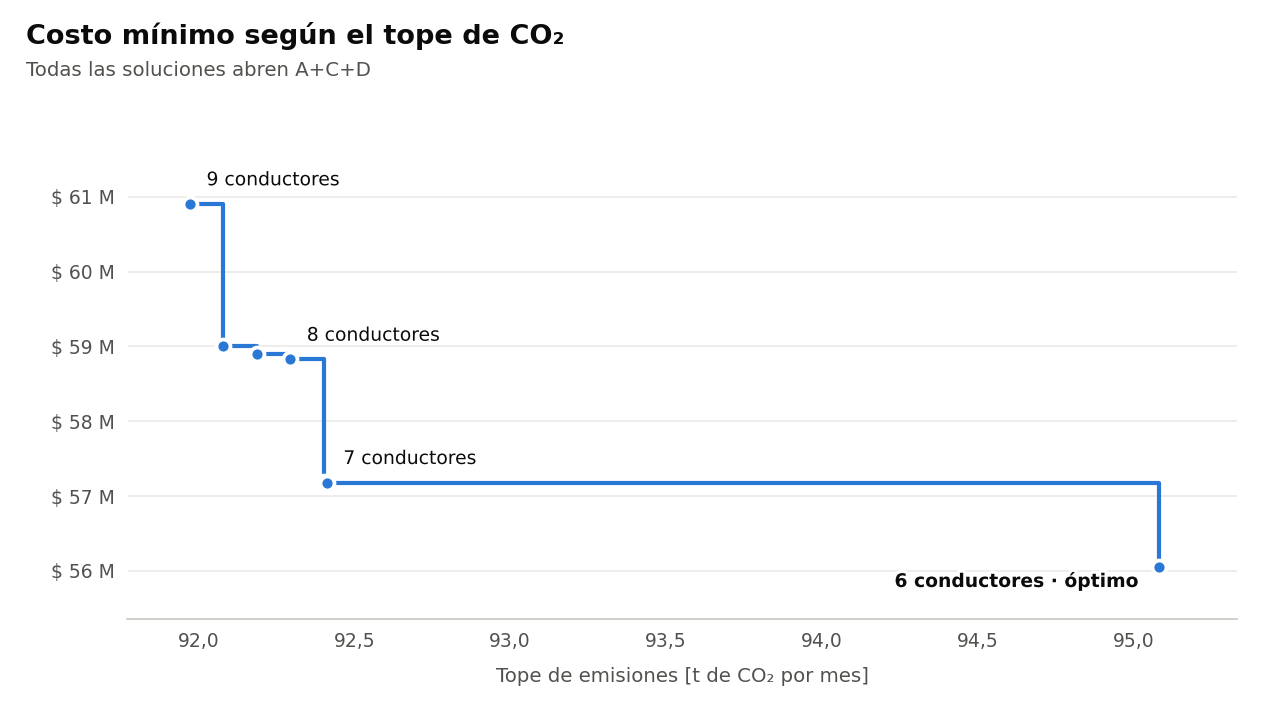
\includegraphics[width=0.82\linewidth]{../resultados/graficos/01_frontera_costo_co2.png}
\caption{Costo mínimo para cada tope de emisiones. Con conductores enteros, la
frontera es una escalera: cada escalón es un conductor más.}
\label{fig:frontera}
\end{figure}

Todas las soluciones de la frontera abren A+C+D. El margen de reducción es
estrecho: el mínimo posible es 91.973\,kg de CO$_2$ por mes, un 3,3\,\% menos
que el óptimo de costo, y alcanzarlo cuesta \$\,4,85 millones más (8,7\,\%),
unos \$\,1.560 por kilogramo evitado. El primer escalón es el más eficiente:
2,7 toneladas menos por \$\,1,13 millones, unos \$\,420 por kilogramo. El
mecanismo es siempre el mismo: bajar emisiones exige trasladar kilómetros del
tramo tercerizado, que cuesta \$\,250 por kilómetro físico, al propio, que cuesta
\$\,325 de combustible más la fracción de conductor.

% ============================================================================
\section{Análisis de sensibilidad}
\label{sec:sensibilidad}

Un modelo con variables enteras no admite análisis post-óptimo: los precios
sombra y los rangos provienen de la base óptima de un problema lineal, y el
óptimo entero no tiene una base asociada \cite{catedra-mip}. La salida
adoptada tiene dos partes:

\begin{enumerate}
  \item \textbf{Sobre la decisión de flujos}: se fijan las variables enteras
  en su valor óptimo —A, C y D abiertos, gerente, 6 conductores— y queda un
  problema lineal de transbordo, sobre el que se calculan los rangos clásicos
  \cite{catedra-sens}. Para ello el mismo modelo de PuLP se exportó y se
  resolvió con HiGHS \cite{highs}, que informa los rangos de lados derechos y
  de costos; el costo coincide con el de CBC al centavo.
  \item \textbf{Sobre la decisión de localización}: lo que puede cambiar qué
  centros se abren se evalúa resolviendo nuevamente el modelo entero en un
  barrido de parámetros (Sección~\ref{sec:barridos}) y bajo cada supuesto
  alternativo (Sección~\ref{sec:tests}).
\end{enumerate}

\subsection{Rangos de nivel de actividad}
\label{sec:b1}

El precio sombra de un recurso indica cuánto cambia el costo por cada unidad
adicional de ese recurso, y el rango indica entre qué valores del lado derecho
ese precio sigue siendo válido.

\begin{table}[H]
\centering\small
\caption{Recursos del problema de flujos con la configuración óptima fija.
Precio negativo: una unidad más del recurso \emph{reduce} el costo.}
\label{tab:rhs}
\begin{tabular}{lrrrl}
\toprule
\textbf{Recurso} & \textbf{Disponible} & \textbf{Usado} & \textbf{Precio sombra} & \textbf{Rango de validez} \\
\midrule
Capacidad de A                 & 40.000 & 31.481 & 0              & [31.481; $\infty$) \\
Capacidad de C                 & 15.000 & 10.369 & 0              & [10.369; $\infty$) \\
\cuello{Capacidad de D}        & 10.000 & 10.000 & \cuello{$-$\$\,265,8 por pallet} & [9.820; 10.670] \\
\cuello{km de los conductores} & 46.200 & 46.200 & \cuello{$-$\$\,222,3 por km}     & [45.960; 47.273] \\
\bottomrule
\end{tabular}
\end{table}

\textbf{Los cuellos de botella son dos: la capacidad de D y los kilómetros de
los conductores.} Un pallet más de capacidad en D ahorraría \$\,266 por mes,
hasta 670 pallets adicionales: D atiende la zona sur, y cada pallet que no
puede atender lo entrega A, desde más lejos. Un
kilómetro más de manejo ahorraría \$\,222. Conviene notar que 7.700\,km a
\$\,222 suman \$\,1,71 millones, más que el costo de un conductor
(\$\,1,6 millones); sin embargo el modelo entero no contrata un séptimo
conductor, porque el precio solo es válido hasta 1.073\,km adicionales y más
allá el ahorro marginal cae. Es exactamente la advertencia de la teoría: fuera
del rango el precio sombra deja de valer y hay que resolver de nuevo
\cite{catedra-sens}.

\paragraph{Costo marginal de servir.} El precio sombra de cada restricción de
demanda (R1) es el costo de abastecer un pallet más de ese producto en ese
supermercado.

\begin{table}[H]
\centering\small
\caption{Costo marginal de un pallet adicional de demanda [\$/pallet].}
\label{tab:marginal}
\setlength{\tabcolsep}{5pt}
\begin{tabular}{lrrrrrrrrrr}
\toprule
\textbf{Producto} & \textbf{S1} & \textbf{S2} & \textbf{S3} & \textbf{S4} & \textbf{S5} & \textbf{S6} & \textbf{S7} & \textbf{S8} & \textbf{S9} & \textbf{S10} \\
\midrule
Fideos     & 1.390 & 510 & 908 & 642 & 659 & 1.134 & 1.072 & 566 & 924 & 650 \\
Arroz      & \textbf{2.228} & 896 & 1.294 & 1.480 & 1.497 & 1.854 & 1.910 & 1.404 & 1.762 & 1.488 \\
Leche      & 1.325 & 640 & 1.038 & 817 & 834 & 1.308 & 969 & 741 & 821 & 825 \\
Gaseosas   & 974 & 1.096 & 1.494 & 546 & 563 & 1.038 & 617 & \textbf{470} & \textbf{470} & 554 \\
Galletitas & 1.640 & 525 & 923 & 891 & 909 & 1.383 & 1.322 & 816 & 1.174 & 900 \\
\bottomrule
\end{tabular}
\end{table}

El rango va de \$\,470 —gaseosas en S8 y S9, cuya planta está junto al
centro D— a \$\,2.228 —arroz en S1, cuya planta está en el extremo noroeste y
el supermercado en el sureste—. Esta tabla es la base de la pregunta~c): es el
costo incremental de servir cada pallet, la referencia contra la cual se
compara cualquier oferta de un tercero.

\subsection{Rangos de soluciones posibles}
\label{sec:b2}

Los rangos de costos indican cuánto puede variar el costo por pallet de cada
arco sin que cambie la solución óptima. De las 171 variables de flujo de los centros abiertos, 67
transportan mercadería. La Tabla~\ref{tab:rangos_costos} muestra los del
tramo de abastecimiento.

\begin{table}[H]
\centering\small
\caption{Rangos de costo de los arcos planta $\to$ centro utilizados [\$/pallet].}
\label{tab:rangos_costos}
\begin{tabular}{llrrrr}
\toprule
\textbf{Planta} & \textbf{Centro} & \textbf{Pallets} & \textbf{Costo actual} & \textbf{Puede bajar} & \textbf{Puede subir} \\
\midrule
Arroz       & A & 5.251  & 1.113,3 & 35,9 & 0 \\
Arroz       & C & 2.319  & 519,7 & 2.404,4 & 124,1 \\
Arroz       & D & 980    & 1.375,6 & 0 & 38,2 \\
Fideos 1    & C & 3.700  & 133,5 & 334,3 & 264,6 \\
Fideos 2    & A & 13.300 & 275,5 & 0 & 38,2 \\
Fideos 2    & D & 3.300  & 537,8 & 38,2 & 0 \\
Galletitas  & A & 5.000  & 525,0 & 0 & 38,2 \\
Galletitas  & C & 1.750  & 148,5 & 99,8 & 1.160,6 \\
Galletitas  & D & 1.750  & 787,3 & 38,2 & 0 \\
Gaseosas    & A & 2.380  & 179,4 & 244,2 & 373,2 \\
Gaseosas    & C & 900    & 719,2 & 1.016,1 & 244,2 \\
Gaseosas    & D & 1.270  & 83,0 & 373,2 & 320,4 \\
Leche 1     & D & 2.700  & 434,5 & 453,8 & 239,9 \\
Leche 2     & A & 5.550  & 450,3 & 239,9 & 235,8 \\
Leche 2     & C & 1.700  & 263,2 & 289,2 & 848,4 \\
\bottomrule
\end{tabular}
\end{table}

Se observan dos fenómenos. El primero es la \textbf{degeneración}, típica de
los problemas de transbordo: seis arcos no admiten ningún aumento de costo y
cuatro no admiten ninguna baja sin que cambie la solución. El arco de la planta
de fideos más cercana a A, con 13.300 pallets, es el más importante de la red,
y un aumento de apenas \$\,38 por pallet ya modifica el reparto. El valor
\$\,38,2 se repite porque esos arcos compiten entre sí por la capacidad de D:
encarecer uno desplaza mercadería hacia otro.

El segundo son los \textbf{óptimos alternativos}. De los 104 arcos sin uso,
dos tienen costo reducido nulo: A $\to$ S7 para fideos y para galletitas. El
costo del tramo propio no depende del producto, de modo que, en un par
centro–supermercado, el reparto entre productos puede variar sin cambiar el
costo; el total transportado en cada par, en cambio, es único. Los arcos más
próximos a entrar en la solución son D $\to$ S1 (costo reducido de \$\,38 por
pallet) y A $\to$ S9 (\$\,41): son los supermercados de la frontera entre las
zonas de A y de D.

\paragraph{Control cruzado.} Los precios y rangos de HiGHS se verificaron en
nueve casos, cambiando el dato en el modelo original y resolviendo de nuevo:
por ejemplo, ampliar D en 603 pallets (dentro del rango) baja el costo
\$\,265,80 por pallet, exactamente el precio sombra, y ampliarlo en 1.005
(fuera del rango) da \$\,253,05. Todos los casos coinciden.

\subsection{Barridos sobre la decisión de localización}
\label{sec:barridos}

Los rangos anteriores suponen la configuración fija. Lo que puede cambiar qué
centros se abren se evaluó resolviendo el modelo entero para cada valor de
cuatro parámetros (Figura~\ref{fig:barridos}).

\begin{figure}[H]
\centering
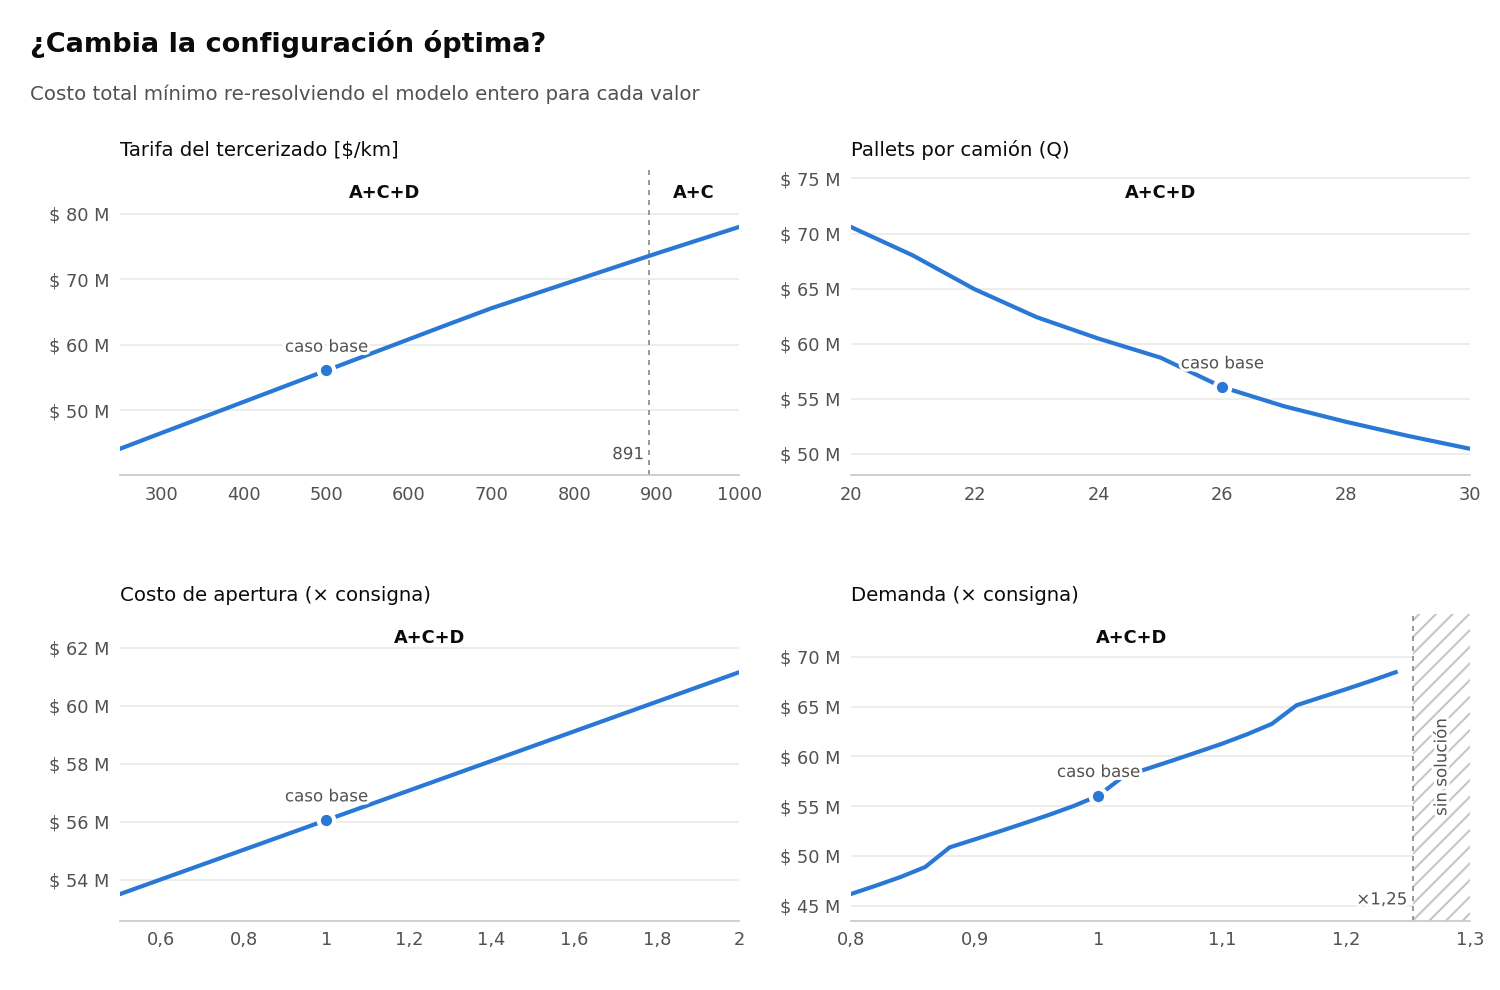
\includegraphics[width=0.95\linewidth]{../resultados/graficos/04_barridos.png}
\caption{Costo total óptimo al barrer cada parámetro, con la configuración
óptima rotulada en cada tramo.}
\label{fig:barridos}
\end{figure}

\begin{itemize}
  \item \textbf{Tarifa del tercerizado.} A+C+D es óptima hasta \$\,890,8 por
  kilómetro, un 78\,\% por encima de la tarifa actual. Con una tarifa mayor
  conviene A+C: sin D, el tramo tercerizado es más corto porque las plantas
  están al norte.
  \item \textbf{Pallets por camión.} Entre 20 y 30 pallets la configuración no
  cambia. Es, sin embargo, el parámetro que más mueve el costo
  (de \$\,70,6 a \$\,50,5 millones) y las emisiones (de 122 a 80 toneladas):
  la carga del camión determina directamente cuántos viajes se hacen.
  \item \textbf{Costo de apertura.} Entre la mitad y el doble, sin cambios.
  \item \textbf{Demanda.} A+C+D sostiene un crecimiento de hasta el 25,4\,\%
  (65.000 pallets, su capacidad conjunta); más allá el modelo no tiene
  solución bajo S2, y habría que admitir A y B abiertos a la vez.
\end{itemize}

\subsection{Sensibilidad a los supuestos}
\label{sec:tests}

Cada supuesto con lectura alternativa se evaluó cambiándolo de a uno y
resolviendo el modelo entero completo (Tabla~\ref{tab:tests}).

\begin{table}[H]
\centering\footnotesize
\caption{Resultado de los tests de supuestos.}
\label{tab:tests}
\begin{tabularx}{\linewidth}{@{}llllX@{}}
\toprule
\textbf{Test} & \textbf{Supuesto} & \textbf{Alternativa} & \textbf{Configuración} & \textbf{Efecto} \\
\midrule
A & S1 Distancias        & Línea recta × 1,27     & A+C+D & +1,8\,\% de costo, +2,7\,\% de CO$_2$ \\
B & S2 Principal         & A y B permitidos       & A+C+D & Ninguno: abrir A y B nunca conviene \\
C & S5 Camión            & 20 a 30 pallets        & A+C+D & De +26\,\% a $-$10\,\% de costo \\
D & S6 Tarifa            & Sobre ida y vuelta     & \textbf{A+C} & +38,9\,\% de costo \\
E & S7 Sueldo            & ±30\,\%                & A+C+D & ±5,1\,\% de costo \\
E & S7 km por conductor  & 6.000 a 12.000         & A+C+D & De +5,1\,\% a $-$6,3\,\% (8 a 4 conductores) \\
F & S9 Carbono           & USD 10, 50 y 100 por t & A+C+D & Ninguno: no cambian ni los flujos \\
G & S10 Apertura         & ×0,05 a ×2             & A+C+D & De $-$8,6\,\% a +9,1\,\% de costo \\
\bottomrule
\end{tabularx}
\end{table}

La configuración A+C+D resiste todos los supuestos salvo uno. El test~D
duplica el costo del tramo tercerizado, lo que equivale a una tarifa de
\$\,1.000 por kilómetro de ida, por encima del umbral hallado en la
Sección~\ref{sec:barridos}: en ese caso conviene A+C, coherente con el
barrido. \textbf{La recomendación de abrir A, C y D no depende, por lo tanto,
de los datos externos incorporados} —el camión, el sueldo y el recorrido de
los conductores, el factor de emisión— ni de que la apertura sea un costo
mensual o una inversión amortizada en muchos meses (test~G); depende de cómo
se pacte la tarifa con el tercerizado.

El test~F merece una mención: aun con un precio del carbono de USD\,100 por
tonelada, diez veces el de la ley argentina \cite{ley27430}, el óptimo no
cambia. La razón está en la frontera de la Sección~\ref{sec:frontera}: evitar
un kilogramo de CO$_2$ cuesta al menos \$\,420, y USD\,100 por tonelada son
\$\,155 por kilogramo al tipo de cambio oficial \cite{bna}.

% ============================================================================
\section{Representación gráfica del flujo de los transportes}
\label{sec:grafica}

La Figura~\ref{fig:esquema} resume la estructura de la red y las tres
decisiones del modelo; la Figura~\ref{fig:flujos_a} muestra los flujos de la
solución óptima.

\begin{figure}[H]
\centering
\resizebox{\linewidth}{!}{%
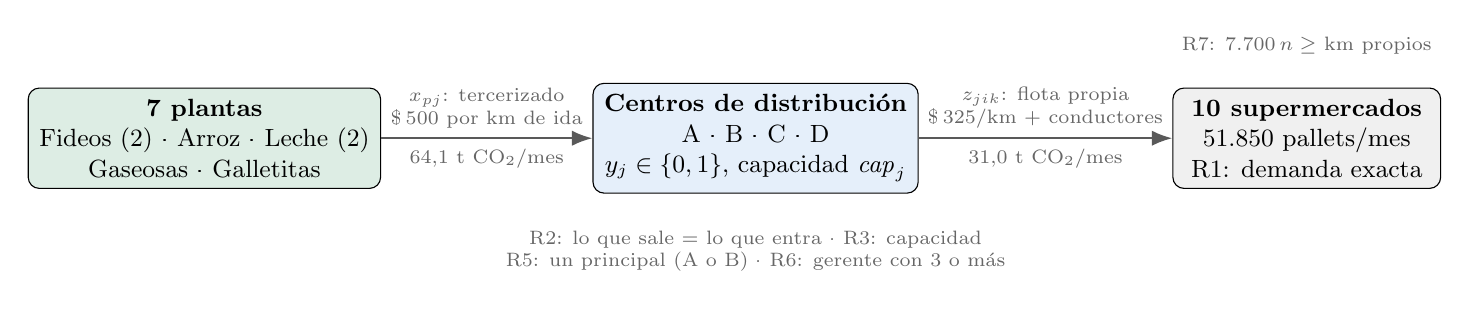
\begin{tikzpicture}[
  box/.style={draw, rounded corners, align=center, minimum height=1.0cm, font=\small, inner sep=4pt},
  arrow/.style={-{Latex[length=2.6mm]}, thick, color=black!65},
  tag/.style={font=\scriptsize, align=center, text=black!60}
]
\node[box, fill=planta!15, minimum width=3.4cm] (pl) at (0,0)
  {\textbf{7 plantas}\\Fideos (2) · Arroz · Leche (2)\\Gaseosas · Galletitas};
\node[box, fill=centroA!12, minimum width=3.6cm] (cd) at (7,0)
  {\textbf{Centros de distribución}\\A · B · C · D\\$y_j \in \{0,1\}$, capacidad $\mathit{cap}_j$};
\node[box, fill=black!6, minimum width=3.4cm] (su) at (14,0)
  {\textbf{10 supermercados}\\51.850 pallets/mes\\R1: demanda exacta};
\draw[arrow] (pl) -- node[tag, above] {$x_{pj}$: tercerizado\\\$\,500 por km de ida} node[tag, below] {64,1 t CO$_2$/mes} (cd);
\draw[arrow] (cd) -- node[tag, above] {$z_{jik}$: flota propia\\\$\,325/km + conductores} node[tag, below] {31,0 t CO$_2$/mes} (su);
\node[tag, below=0.35cm of cd] {R2: lo que sale = lo que entra · R3: capacidad\\R5: un principal (A o B) · R6: gerente con 3 o más};
\node[tag, above=0.3cm of su] {R7: $7.700\,n \geq$ km propios};
\end{tikzpicture}}
\caption{Estructura de la red de distribución, con las variables de cada
tramo, sus costos y sus emisiones en la solución óptima.}
\label{fig:esquema}
\end{figure}

\begin{figure}[H]
\centering
\begin{subfigure}[b]{0.55\linewidth}
\centering
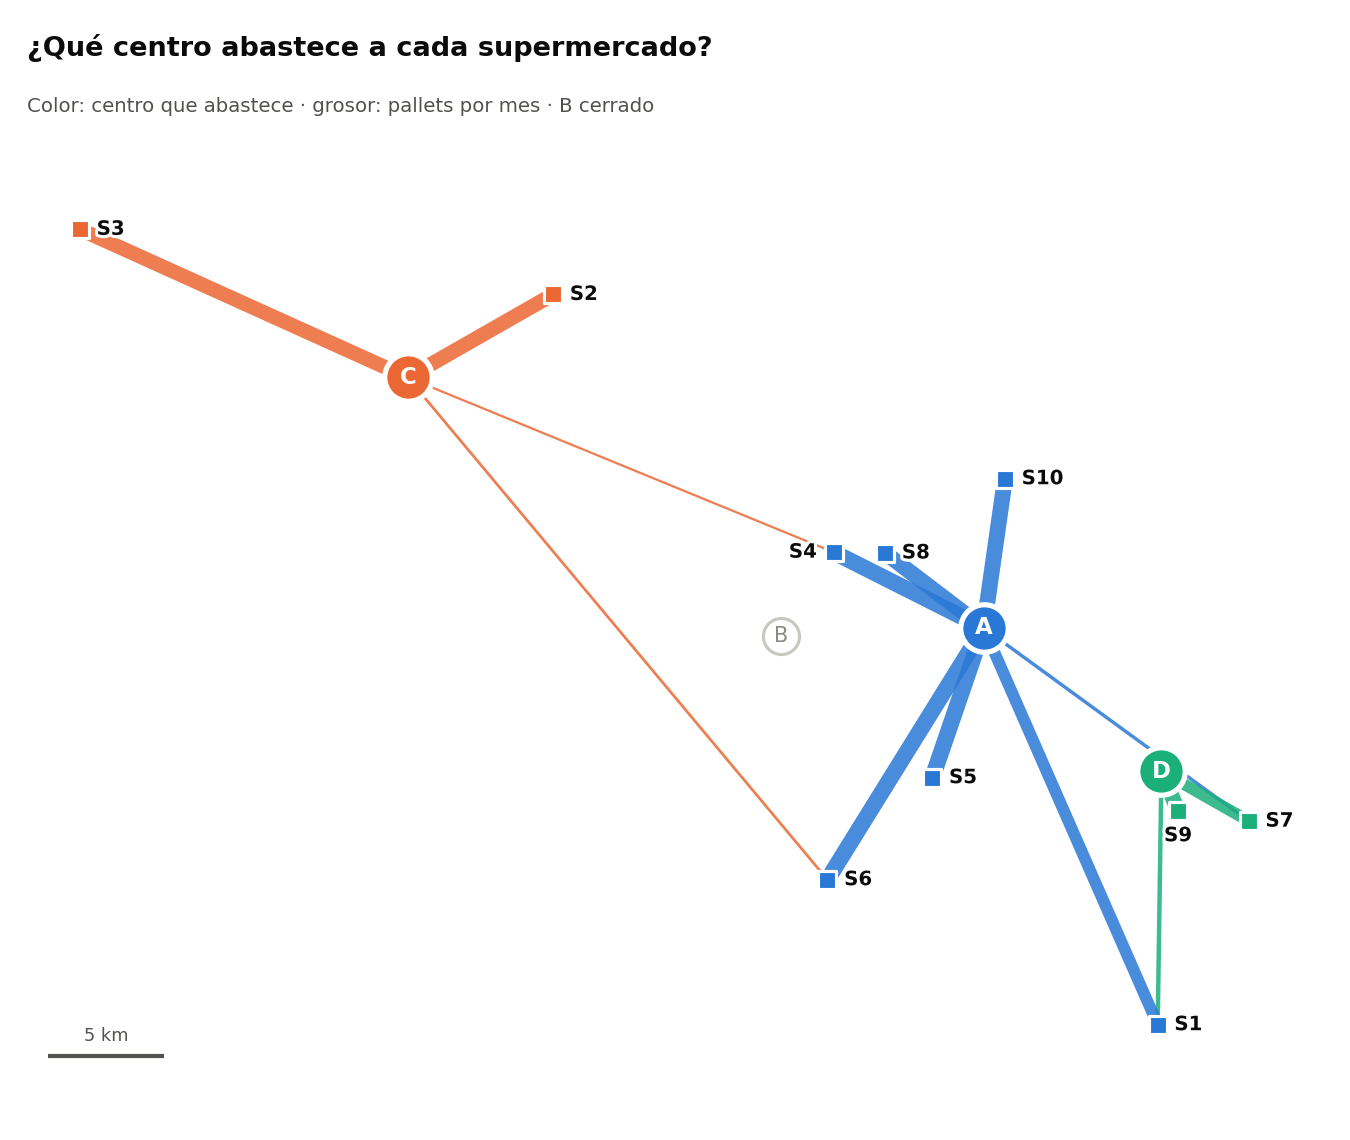
\includegraphics[width=\linewidth]{../resultados/graficos/02_mapa_flujos_a.png}
\caption{Centro $\to$ supermercado: color del centro que abastece, grosor
proporcional a los pallets.}
\label{fig:mapa_a}
\end{subfigure}\hfill
\begin{subfigure}[b]{0.42\linewidth}
\centering
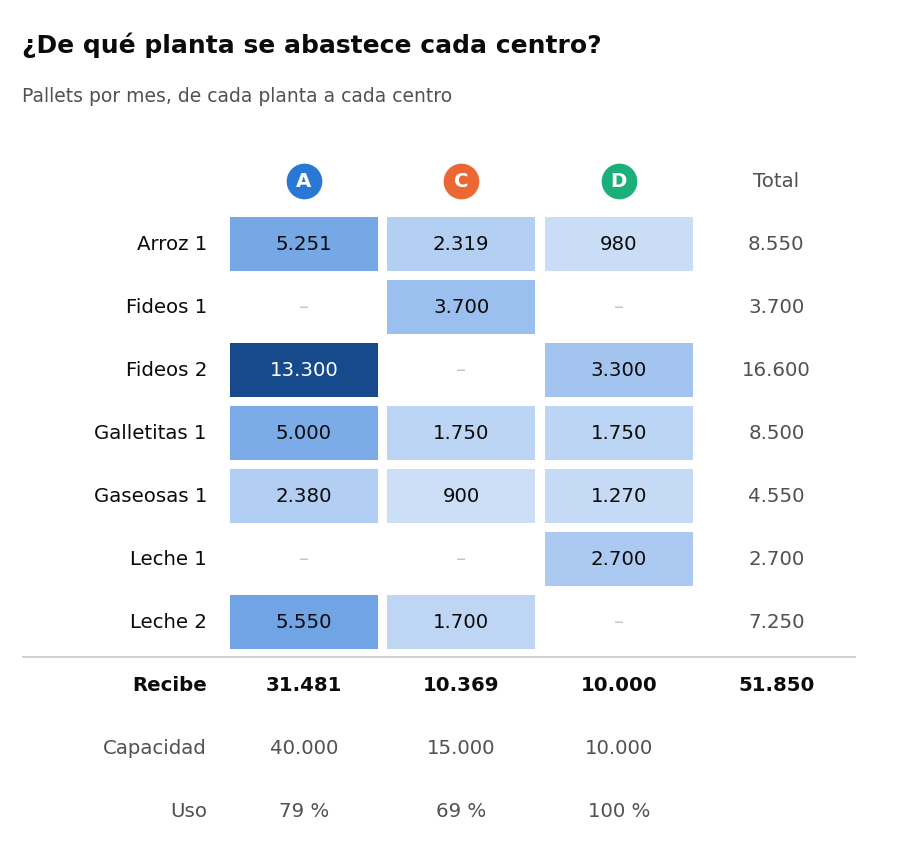
\includegraphics[width=\linewidth]{../resultados/graficos/03_tabla_tramo1_a.png}
\caption{Planta $\to$ centro, en pallets por mes.}
\label{fig:tramo1_a}
\end{subfigure}
\caption{Flujos de la solución óptima. Los quince flujos de planta a centro se
leen mejor como tabla que como flechas sobre el mapa.}
\label{fig:flujos_a}
\end{figure}

Los mismos gráficos para la pregunta~d) se presentan en su sección.

% ============================================================================
\section{Librerías utilizadas}
\label{sec:librerias}

El trabajo se desarrolló en Python con el siguiente conjunto de herramientas:

\begin{itemize}
  \item \textbf{PuLP} \cite{pulp} con el solver \textbf{CBC} \cite{cbc}: modelado y
  resolución del modelo entero mixto, por \emph{Branch \& Bound}.
  \item \textbf{highspy}, la interfaz de Python del solver \textbf{HiGHS}
  \cite{highs}: rangos de sensibilidad del problema de flujos
  (\texttt{getRanging}), que PuLP no informa. El modelo de PuLP se exportó en
  formato MPS para resolver exactamente el mismo problema.
  \item \textbf{SciPy} \cite{scipy}: optimización continua del punto de Weber de
  la pregunta~b) (\texttt{scipy.optimize.minimize}, método de Nelder–Mead).
  \item \textbf{requests}, para consultar una única vez el servicio
  \texttt{table} de \textbf{OSRM} \cite{osrm} (matriz de distancias por calle) y
  el servicio de \textbf{Nominatim} \cite{nominatim} (nombre de la zona de un
  punto). Las respuestas quedan guardadas, de modo que los cálculos se
  reproducen sin conexión.
  \item \textbf{pandas} y \textbf{NumPy}: tablas de datos y de resultados.
  \item \textbf{matplotlib}: todos los gráficos; el esquema de la
  Figura~\ref{fig:esquema} está hecho con Ti\emph{k}Z.
\end{itemize}

Como en los trabajos anteriores, el modelo se escribió \textbf{una sola vez},
como función parametrizada:
\begin{quote}
\centering\small
\texttt{resolver(params, escenario, config\_fija, epsilon\_co2, goyito, objetivo, fijar\_n)}
\end{quote}
El caso base, la enumeración de configuraciones, la frontera costo–emisiones,
el problema de flujos de la sensibilidad, los barridos, los tests y las
preguntas~c), d) y~e) son llamadas a esa misma función con otros argumentos.
Los supuestos residen en un único diccionario de configuración, y un supuesto
inexistente o fuera de rango produce un error en lugar de devolver el caso
base en silencio. La única excepción es la pregunta~b), que cambia la
naturaleza del problema —la ubicación pasa a ser continua— y tiene su propio
módulo.

% ============================================================================
\section{Respuestas a las preguntas de la consigna}
\label{sec:preguntas}

\subsection{a) Localización óptima de los centros de distribución}
\label{sec:pa}

\textbf{Conviene abrir los centros A, C y D}, con un gerente de coordinación y
seis conductores propios, a un costo de \textbf{\$\,56,06 millones por mes}.
La red consume \textbf{35.478 litros de gasoil} y emite \textbf{95,1 toneladas
de CO$_2$} por mes, dos tercios de ellas en el tramo tercerizado.

La Tabla~\ref{tab:configuraciones} cuantifica las tres configuraciones
posibles. A+C+D es a la vez la más barata y la de menores emisiones, de modo
que en esta decisión \textbf{no hay conflicto entre el criterio económico y el
ambiental}: la configuración que ahorra kilómetros ahorra pesos y emisiones.
El conflicto aparece en un segundo nivel, el reparto de los flujos dentro de
A+C+D, y es acotado: las emisiones pueden reducirse a lo sumo un 3,3\,\%, a
un costo creciente que parte de \$\,420 por kilogramo evitado
(Sección~\ref{sec:frontera}).

\subsection{b) Un único centro de capacidad infinita y costos nulos}
\label{sec:pb}

Sin capacidad ni costos fijos, el problema deja de ser una elección entre
cuatro candidatos y se convierte en un \textbf{problema de Weber}: ubicar en
cualquier punto del mapa el centro que minimice la suma de distancias
ponderadas a las plantas y a los supermercados:
\[
\text{Min}_{X}\; \sum_k a\,\frac{\mathit{dem}_k}{Q} \min_{p \in P_k} d(p, X)
\;+\; \sum_i b\,\frac{\mathit{dem}_i}{Q}\, 2\, d(X, i)
\]
con dos juegos de pesos. En el \textbf{criterio económico}, $a = \$\,500$ por
kilómetro de ida del tercerizado y $b = \$\,325 + W/K_{\max} = \$\,533$ por
kilómetro físico propio, con el conductor expresado como costo por kilómetro.
En el \textbf{criterio ambiental}, la función son los kilómetros físicos
totales, que determinan directamente el gasoil y las emisiones. El mínimo sobre
las plantas —la de fideos y la de leche pueden cambiar según dónde esté el
centro— hace que la función no sea convexa; por eso se resolvió en dos etapas.

\paragraph{Etapa 1: la zona.} Con distancias en línea recta por el factor de
ruta, una búsqueda en grilla refinada con Nelder–Mead ubica el óptimo
económico en el límite entre General San Martín y la Ciudad, a pocos metros
del supermercado S4, y el ambiental 5\,km más al norte. El algoritmo de
Weiszfeld \cite{weiszfeld}, resuelto en forma independiente, coincide a menos
de 15 metros.

\paragraph{Etapa 2: el punto concreto, por calle.} El factor de ruta es un
promedio, y la red real no es uniforme: alrededor del óptimo de la etapa~1 las
calles resultaron 1,5 veces más largas que la línea recta, y por calle ese
punto sale un 10,7\,\% más caro que el mejor. La respuesta se determinó por
eso sobre la red real: 336 puntos candidatos cada 1\,km en la zona central,
con distancias por calle de OSRM; se descartaron 33 que no quedan a menos de
300\,m de una calle.

\begin{table}[H]
\centering\small
\caption{Centro único: costo de transporte y emisiones mensuales, con distancias por calle.}
\label{tab:pb}
\begin{tabular}{lrrrrr}
\toprule
\textbf{Ubicación} & \textbf{Costo [\$/mes]} & \textbf{Sobrecosto} & \textbf{Conduct.} & \textbf{km} & \textbf{kg CO$_2$} \\
\midrule
\textbf{Óptimo económico (Villa Urquiza)} & \textbf{61.019.265} & --- & 10 & 157.684 & 105.649 \\
Óptimo ambiental (Villa Adelina)          & 65.501.331 & +7,3\,\% & 13 & 150.697 & 100.967 \\
Centro A                                  & 64.916.011 & +6,4\,\% & 10 & 172.771 & 115.757 \\
Centro B                                  & 75.268.449 & +23,4\,\% & 12 & 195.775 & 131.169 \\
Centro C                                  & 83.578.568 & +37,0\,\% & 17 & 188.332 & 126.183 \\
Centro D                                  & 85.584.233 & +40,3\,\% & 13 & 232.012 & 155.448 \\
\bottomrule
\end{tabular}
\end{table}

\textbf{El centro único debería ubicarse en el noroeste de la Ciudad, en la
zona de Villa Urquiza} (punto óptimo: $-34{,}57$; $-58{,}48$), cerca del
límite con el conurbano norte. Los cuatro candidatos que quedan a menos del
1\,\% del óptimo están todos en esa zona, en un radio de unos 4\,km. La
justificación es económica y ambiental a la vez: el punto equilibra el
abastecimiento desde las plantas del norte y el noroeste con la entrega a los
supermercados, concentrados en el centro y el sur, y tiene una buena conexión
con la red de calles: desde allí, los recorridos reales son en promedio 1,24
veces la línea recta, contra 1,49 desde el óptimo de la etapa~1.

\begin{figure}[H]
\centering
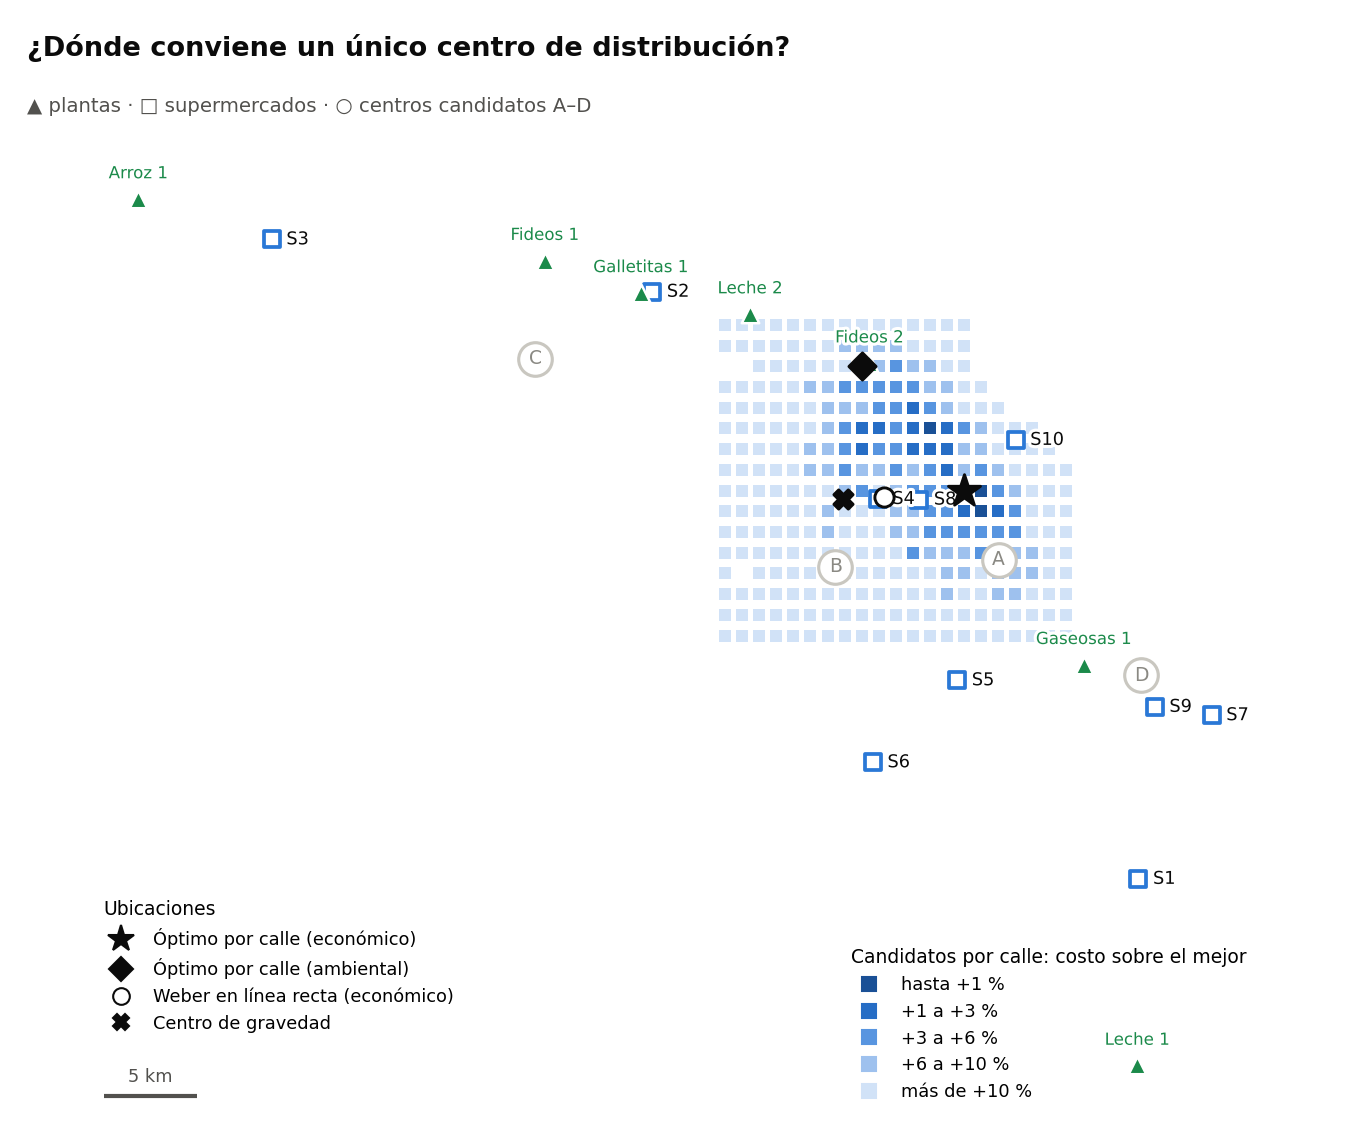
\includegraphics[width=0.72\linewidth]{../resultados/graficos/05_mapa_punto_b.png}
\caption{Candidatos para un centro único, coloreados según cuánto más caros
que el mejor resultan con distancias por calle. Los más convenientes forman
una franja entre el noroeste de la Ciudad y el norte del conurbano.}
\label{fig:mapa_b}
\end{figure}

Entre los criterios hay una diferencia que conviene explicitar. El óptimo
ambiental, 8,6\,km al noroeste, recorre un 4,4\,\% menos de kilómetros
(4,7 toneladas menos de CO$_2$ por mes), pero cuesta un 7,3\,\% más, porque
traslada recorrido desde el tramo tercerizado, que cuesta \$\,250 por
kilómetro físico, al tramo propio, que cuesta \$\,533. El centro de gravedad
—el promedio ponderado de las coordenadas, la respuesta intuitiva— queda
2,2\,km al oeste del óptimo de la etapa~1 y resulta un 2,5\,\% más caro. Entre
los candidatos originales, solo A se acerca al óptimo (+6,4\,\%).

\paragraph{Comparación con la red de la pregunta a).} Aun sin pagar apertura
ni operación, el centro único es más caro que la red A+C+D: su transporte
cuesta \$\,61,0 millones por mes, frente a \$\,48,5 millones de transporte de
A+C+D (+25,8\,\%), recorre 15.774\,km más (+11,1\,\%) y emite 10,6 toneladas
más de CO$_2$ por mes. Incluso sumando a la red sus \$\,7,6 millones de costos
fijos y de operación, la descentralización resulta más barata. \textbf{Con
plantas y supermercados dispersos en un área de 60\,km, un centro único,
aunque sea gratuito, obliga a recorrer más kilómetros que tres centros bien
ubicados.}

\subsection{c) Precio mínimo de Goyito por producto}
\label{sec:pc}

Goyito ofrece transportar cada producto directamente desde la planta hasta el
supermercado, a un precio por pallet entregado. La pregunta es a partir de qué
precio deja de convenir el centro propio. Para cada producto $k$ se resolvió el
modelo completo sin ese producto, $Z^{*}(\text{sin } k)$, y el precio umbral
resulta:
\[
g^{*}_k \;=\; \frac{Z^{*} - Z^{*}(\text{sin } k)}{\mathit{dem}_k}
\]
Si Goyito ofrece transportar el producto $k$ por menos de $g^{*}_k$ por pallet,
conviene tercerizarlo. El resultado se verificó con el modelo entero,
incorporando la opción de Goyito como una variable binaria $u_k$: con un
precio \$\,2 por debajo del umbral, el modelo terceriza el producto; con uno
\$\,2 por encima, no.

\begin{figure}[H]
\centering
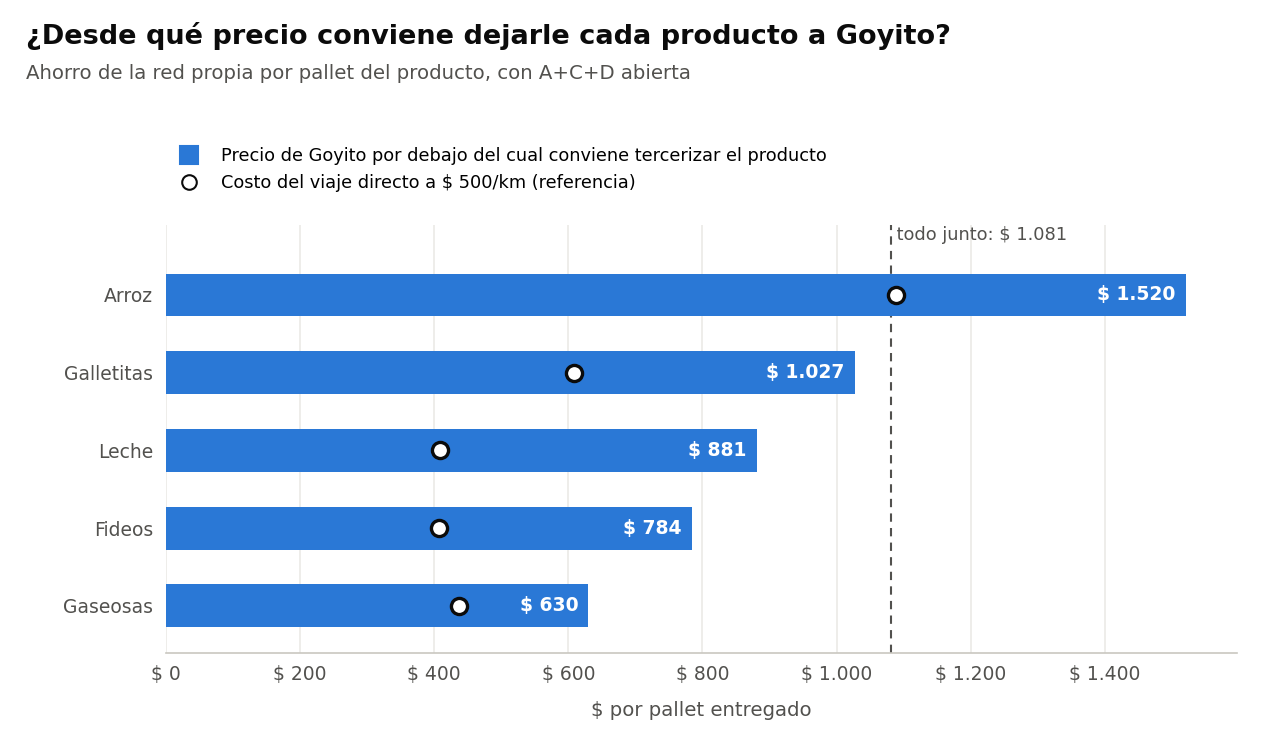
\includegraphics[width=0.84\linewidth]{../resultados/graficos/06_umbral_goyito.png}
\caption{Precio umbral de Goyito por producto, con el costo que tendría el
viaje directo a la tarifa de mercado como referencia.}
\label{fig:goyito}
\end{figure}

\begin{table}[H]
\centering\small
\caption{Precio umbral de Goyito por producto [\$/pallet].}
\label{tab:goyito}
\begin{tabular}{lrrrrr}
\toprule
\textbf{Producto} & \textbf{Demanda} & \textbf{Umbral} & \textbf{Con carbono} & \textbf{Directo a \$\,500/km} & \textbf{Margen} \\
\midrule
Gaseosas   & 4.550  & 630   & 637   & 437   & 193 \\
Fideos     & 20.300 & 784   & 791   & 407   & 378 \\
Leche      & 9.950  & 881   & 890   & 408   & 472 \\
Galletitas & 8.500  & 1.027 & 1.033 & 608   & 419 \\
Arroz      & 8.550  & 1.520 & 1.527 & 1.089 & 432 \\
\midrule
\textbf{Todos, precio único} & \textbf{51.850} & \textbf{1.081} & \textbf{1.086} & 555 & 526 \\
\bottomrule
\end{tabular}
\end{table}

\paragraph{Lectura de los umbrales.} Los umbrales reflejan la geografía: el
arroz tiene el más alto (\$\,1.520) porque su única planta está en el extremo
noroeste y cada pallet recorre la red completa; las gaseosas, el más bajo
(\$\,630), porque su planta está junto a D. Para que \textbf{no resulte viable
instalar el centro}, Goyito debería ofrecer el conjunto de los productos por
menos de \textbf{\$\,1.081 por pallet} en promedio. La suma de los umbrales por
producto (\$\,49,3 millones) es menor que el costo de la red (\$\,56,1
millones): la diferencia, \$\,6,8 millones, es aproximadamente el costo de
apertura y del gerente, que no depende de ningún producto en particular. Por
eso, tercerizar productos sueltos no permite cerrar ningún centro —en los cinco
casos la red sigue siendo A+C+D— y el ahorro de cada producto se limita a su
transporte y a algunos conductores.

\paragraph{Costos ambientales.} El viaje directo de Goyito evita el paso por el
centro: \textbf{recorre 116.152\,km por mes contra 141.910 de la red propia, un
18,2\,\% menos}, y emite 17,3 toneladas menos de CO$_2$ por mes. La reducción
va del 3\,\% en gaseosas, cuya planta está junto a D, al 32\,\% en leche.
Incorporando el CO$_2$ con el precio de la ley argentina
\cite{ley27430} —USD\,10 por tonelada, \$\,15,5 por kilogramo al tipo de
cambio oficial \cite{bna}—, los umbrales suben entre \$\,6 y \$\,10 por pallet:
el beneficio ambiental del viaje directo existe pero, a ese precio, es menor
al 1\,\% del costo.

\paragraph{Advertencia.} La última columna de la Tabla~\ref{tab:goyito} compara
el umbral con lo que costaría el viaje directo a la misma tarifa de mercado de
\$\,500 por kilómetro: entre \$\,407 y \$\,1.089 por pallet. En todos los
productos, ese costo queda por debajo del umbral. Es decir, un operador que
pague la tarifa de mercado podría ofrecer un precio menor que el umbral y aun
así cubrir su transporte: \textbf{la conveniencia del centro propio no se
sostiene en un ahorro de transporte} —el viaje directo es más corto— sino en
el precio que efectivamente cobre Goyito, que incluye su margen y su
estructura. El centro propio se justifica si Goyito cobra más de \$\,1.081 por
pallet en promedio, o por las razones que la propia consigna menciona: la
prioridad que Goyito da a clientes de mayor envergadura y el control de la
cadena de suministro.

\subsection{d) Vehículos propios desde los proveedores}
\label{sec:pd}

Con flota propia también en el tramo de abastecimiento, ese tramo deja de
pagar la tarifa de \$\,500 por kilómetro de ida y pasa a pagar combustible por
la ida y la vuelta, más conductores. En el modelo, el único cambio es el
costo de esos arcos y que sus kilómetros se suman a la restricción R7.

\begin{figure}[H]
\centering
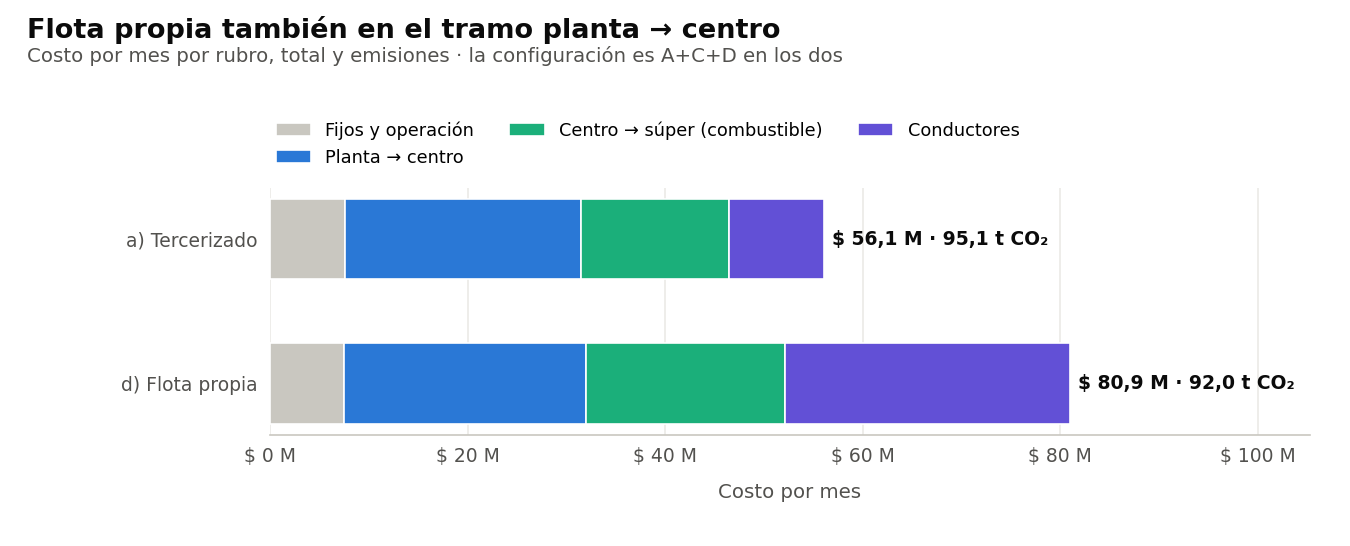
\includegraphics[width=0.78\linewidth]{../resultados/graficos/07_comparacion_a_d.png}
\caption{Costo y emisiones con el tramo de abastecimiento tercerizado (a) y con
flota propia (d).}
\label{fig:comparacion_d}
\end{figure}

\begin{table}[H]
\centering\small
\caption{Comparación entre el escenario actual y la flota propia en los dos tramos.}
\label{tab:pd}
\begin{tabular}{lrrr}
\toprule
\textbf{Indicador} & \textbf{a) Tercerizado} & \textbf{d) Flota propia} & \textbf{Variación} \\
\midrule
Configuración                      & A+C+D      & A+C+D      & --- \\
Costo total [\$/mes]               & 56.055.516 & 80.948.592 & \textbf{+44,4\,\%} \\
\quad Planta $\to$ centro          & 23.893.862 & 24.441.491 & +2,3\,\% \\
\quad Centro $\to$ súper           & 15.015.000 & 20.172.541 & +34,3\,\% \\
\quad Conductores                  & 9.600.000 (6) & 28.800.000 (18) & +200\,\% \\
km por mes                         & 141.910    & 137.274    & $-$3,3\,\% \\
Litros de gasoil por mes           & 35.478     & 34.318     & $-$3,3\,\% \\
kg de CO$_2$ por mes               & 95.080     & 91.974     & \textbf{$-$3,3\,\%} \\
\bottomrule
\end{tabular}
\end{table}

\textbf{El nuevo costo operativo es de \$\,80,9 millones por mes, un 44\,\%
más que el actual}, con la misma configuración. La explicación está en el
costo por kilómetro físico: el tercerizado cuesta \$\,250 (cobra \$\,500 por
el kilómetro de ida e incluye su retorno), mientras que la flota propia cuesta
\$\,325 de combustible más \$\,208 de conductor, \$\,533 en total. La mayor
parte del aumento son conductores: de 6 a 18, \$\,19,2 millones más por mes.

En lo ambiental la flota propia mejora levemente: \textbf{3,3\,\% menos de
kilómetros, de gasoil y de CO$_2$} (3,1 toneladas por mes). Como el camión se
supone el mismo, la mejora no proviene de un vehículo más eficiente sino de
las rutas: cuando todo el transporte es propio, el costo es casi proporcional a
los kilómetros, y minimizar el costo equivale a minimizar el recorrido. De
hecho, las emisiones de d) coinciden con el mínimo de la frontera de la
Sección~\ref{sec:frontera}, que en el escenario actual cuesta \$\,60,9
millones: \textbf{la misma reducción de emisiones se obtiene \$\,20 millones
más barata manteniendo el tercerizado} y reasignando flujos. Cada tonelada de
CO$_2$ evitada con la flota propia cuesta unos \$\,8 millones.

Con flota propia, la diferencia entre configuraciones se reduce: A+C queda a
solo \$\,94.586 de A+C+D (0,1\,\%). La ventaja de abrir D, que en a) era acortar
el tramo propio, pierde peso cuando ambos tramos son igualmente caros por
kilómetro. La propuesta de control del tiempo de llegada, por lo tanto, tiene un
costo concreto: \$\,24,9 millones por mes, que habría que comparar con el valor
operativo de esa previsibilidad.

\begin{figure}[H]
\centering
\begin{minipage}{0.52\linewidth}
\centering
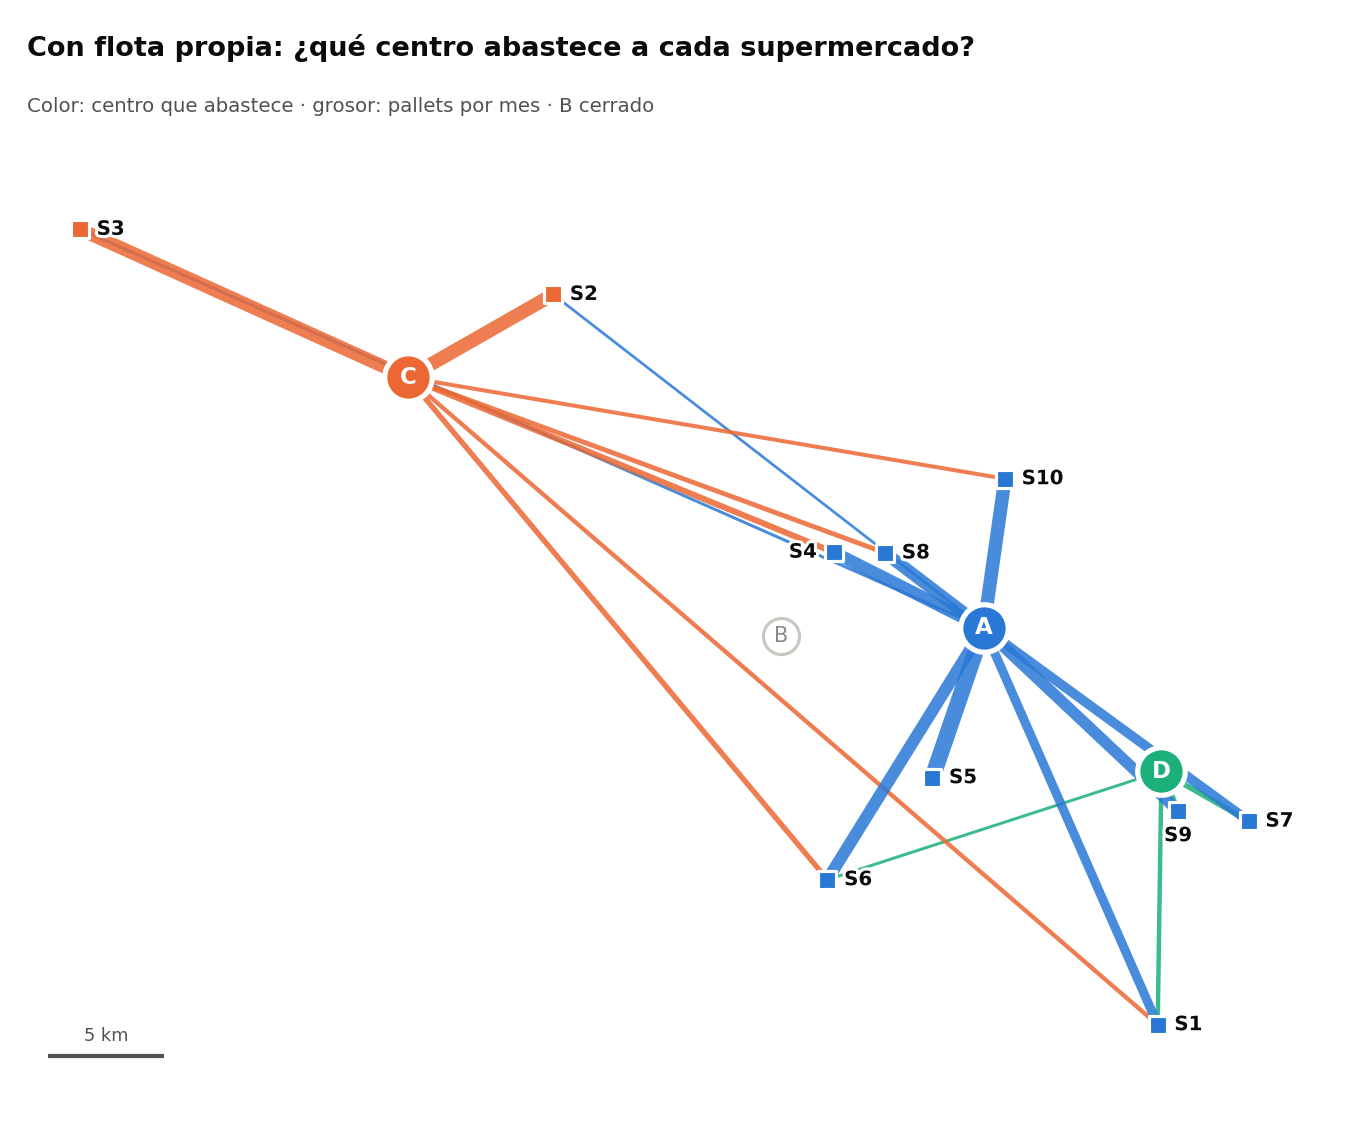
\includegraphics[width=\linewidth]{../resultados/graficos/08_mapa_flujos_d.png}
\end{minipage}\hfill
\begin{minipage}{0.45\linewidth}
\centering
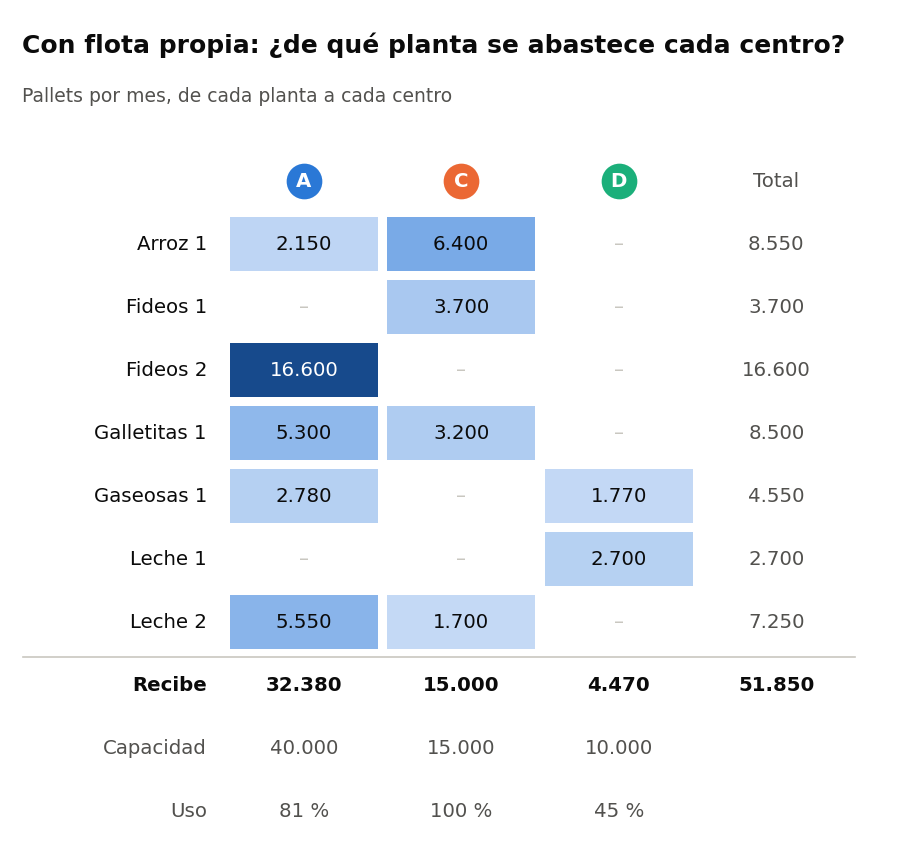
\includegraphics[width=\linewidth]{../resultados/graficos/09_tabla_tramo1_d.png}
\end{minipage}
\caption{Flujos con flota propia en los dos tramos.}
\label{fig:flujos_d}
\end{figure}

\subsection{e) Tope de 500 km por conductor}
\label{sec:pe}

\paragraph{Cómo se incorpora al modelo.} El tope negociado no es una
prohibición sino una meta con penalidad: se puede exceder, pagando \$\,1.000
por kilómetro. Se modela, entonces, con una \textbf{variable de desvío}
\cite{catedra-metas}:
\[
\text{km}_{\text{propios}} - 500\, n \;\leq\; \mathit{exc},
\qquad \mathit{exc} \geq 0,
\qquad \text{Min } Z + 1.000\cdot \mathit{exc}
\]
$\mathit{exc}$ mide los kilómetros que recorre la flota propia por encima de lo
que cubren sus $n$ conductores a 500\,km cada uno, y el funcional los paga. La
restricción de capacidad real de los conductores (R7, 7.700\,km cada uno) se
mantiene: si se reemplazara por el tope, el modelo contrataría cero
conductores y pagaría todos los kilómetros como exceso, una solución sin
sentido físico.

La consigna menciona los kilómetros \cita{recorridos al día} y negocia un
máximo de \cita{500 kilómetros mensuales}. Se adoptó la lectura mensual, que es
la cifra negociada; con 500\,km por día (11.000 por mes) el tope no se activa,
porque ya es mayor que la capacidad real de 7.700\,km.

\begin{figure}[H]
\centering
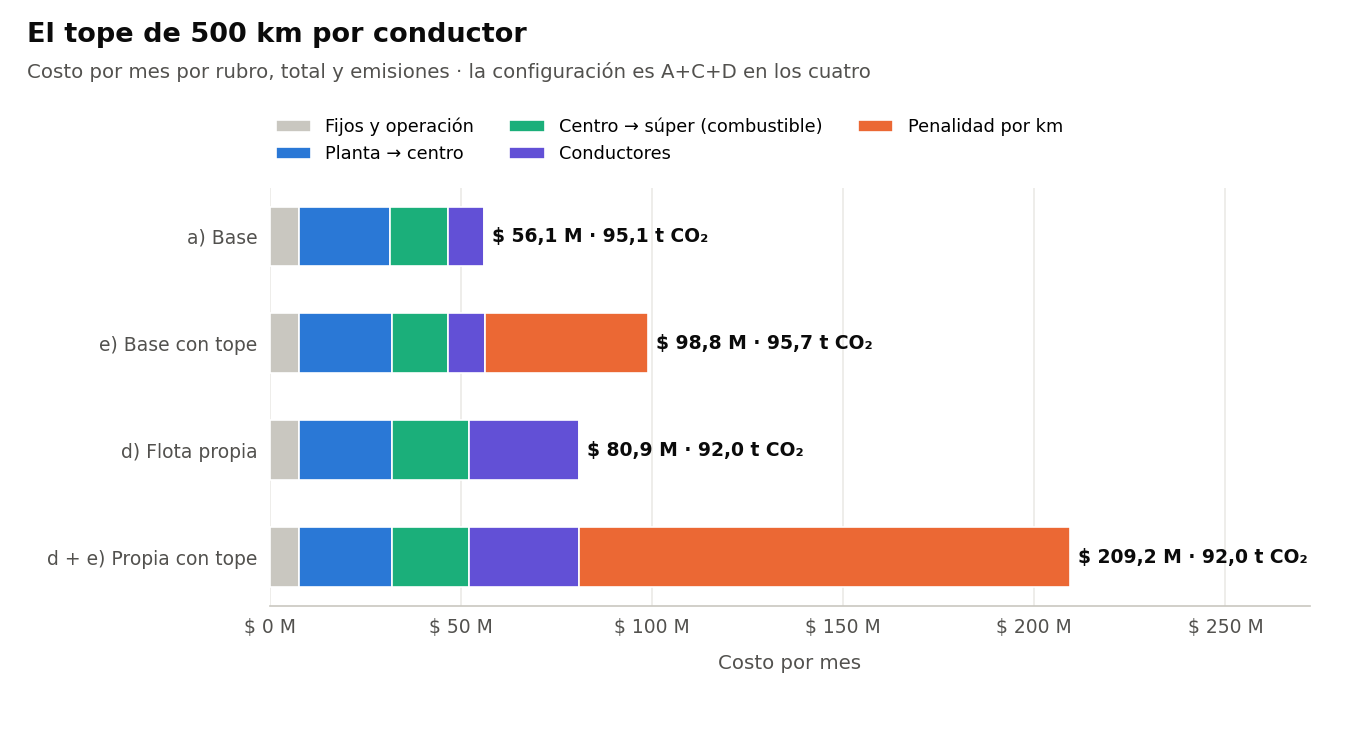
\includegraphics[width=0.74\linewidth]{../resultados/graficos/10_comparacion_e.png}
\caption{Costo por rubro y emisiones con y sin el tope de 500\,km, en el
escenario actual y con flota propia.}
\label{fig:comparacion_e}
\end{figure}

\begin{table}[H]
\centering\small
\caption{Efecto del tope de 500\,km por conductor.}
\label{tab:pe}
\begin{tabular}{lrrrrr}
\toprule
\textbf{Escenario} & \textbf{Costo [\$/mes]} & \textbf{Variación} & \textbf{Conductores} & \textbf{Exceso [km]} & \textbf{kg CO$_2$} \\
\midrule
a) Sin tope                         & 56.055.516  & ---        & 6  & 0       & 95.080 \\
e) Con tope, se paga la penalidad   & \textbf{98.842.374}  & \textbf{+76,3\,\%} & 6  & 42.608  & 95.665 \\
e) Con tope, cumplido contratando   & 193.699.969 & +245,6\,\% & 92 & 0       & 95.236 \\
d) Flota propia, sin tope           & 80.948.592  & +44,4\,\%  & 18 & 0       & 91.974 \\
d + e) Flota propia con tope        & 209.222.470 & +273,2\,\% & 18 & 128.273 & 91.973 \\
\bottomrule
\end{tabular}
\end{table}

\paragraph{Efecto sobre los costos.} Con el tope, el costo sube a
\textbf{\$\,98,8 millones por mes (+76\,\%)}, de los cuales \$\,42,6 millones
son penalidad. El modelo no contrata conductores adicionales, y la razón es
directa: un conductor adicional cuesta \$\,1,6 millones y \emph{cubre}
500\,km, que como exceso costarían \$\,500.000. Mientras el sueldo supere ese
valor, pagar la penalidad es más barato que contratar; un barrido del sueldo
confirma que el comportamiento cambia exactamente en \$\,500.000. Cumplir el
tope sin exceso exigiría 92 conductores y costaría \$\,193,7 millones. Con
flota propia en los dos tramos, donde los kilómetros propios se triplican, el
costo llega a \$\,209 millones. En los cuatro casos la configuración sigue
siendo A+C+D.

\paragraph{Efecto sobre los indicadores ambientales.} El tope encarece cada
kilómetro propio en \$\,1.000 y el modelo reacciona \textbf{trasladando
recorrido al tramo tercerizado}, que no está alcanzado por el acuerdo: el tramo
propio baja de 46.200 a 45.608\,km y el tercerizado sube de 95.710 a
97.175\,km. Como el desvío alarga los recorridos, \textbf{las emisiones
aumentan un 0,6\,\%} (585\,kg de CO$_2$ por mes). Es un caso de ruta forzada en
el sentido de la consigna: una regla laboral que no tiene en cuenta el
ambiente redistribuye el transporte hacia rutas más largas. Con flota propia en
los dos tramos no queda tramo al cual desviar recorrido, y las emisiones no
cambian.

\paragraph{Recomendación.} El tope de 500\,km mensuales equivale a poco más de
un día de trabajo de un conductor, y es incompatible con la operación: su
costo supera al de toda la red. Si el problema es la fatiga, la vía de
negociación que el modelo sugiere es un tope expresado por día o por jornada,
compatible con los 350\,km diarios que el propio convenio toma como referencia.

% ============================================================================
\section{Conclusiones y recomendaciones}
\label{sec:conclusiones}

\begin{table}[H]
\centering\small
\caption{Síntesis de los escenarios analizados.}
\label{tab:sintesis}
\begin{tabular}{llrrr}
\toprule
\textbf{Escenario} & \textbf{Configuración} & \textbf{Costo [\$\,M/mes]} & \textbf{t CO$_2$/mes} & \textbf{Conductores} \\
\midrule
a) Caso base                          & A+C+D        & 56,1  & 95,1  & 6 \\
b) Centro único (solo transporte)     & Villa Urquiza & 61,0  & 105,6 & 10 \\
c) Goyito, viaje directo              & Sin centro   & umbral 1.081 \$/pallet & 77,8 & --- \\
d) Flota propia en los dos tramos     & A+C+D        & 80,9  & 92,0  & 18 \\
e) Tope de 500\,km                    & A+C+D        & 98,8  & 95,7  & 6 \\
\bottomrule
\end{tabular}
\end{table}

\textbf{La localización óptima es robusta.} A, C y D es la mejor configuración
en el caso base, en todos los escenarios de las preguntas, en la frontera
costo–emisiones y bajo todos los supuestos evaluados; solo cambia si se
encarece mucho la tarifa del tercerizado (recomendación~3). La decisión
depende de la geografía —D acorta la entrega a los supermercados del sur— y no
de los datos externos que fue necesario incorporar.

\textbf{El transporte domina el problema.} Representa el 86\,\% del costo, y
dentro de él la tarifa por kilómetro, la carga del camión y la cantidad de
conductores son las palancas reales. La carga del camión, en particular, mueve
el costo en un rango de \$\,20 millones sin modificar la configuración.

\textbf{En la decisión de localización, el criterio económico y el ambiental
coinciden}; en la de flujos, el margen de mejora ambiental es pequeño
(3,3\,\%) y caro (desde \$\,420 por kilogramo). La flota propia alcanza esa
misma reducción, pero cuesta \$\,20 millones más que lograrla con el
tercerizado.

\textbf{El centro propio no se justifica por eficiencia de transporte}: el
viaje directo recorre un 18\,\% menos. Se justifica si Goyito cobra más de
\$\,1.081 por pallet en promedio —con umbrales por producto entre \$\,630 y
\$\,1.520— o por el control de la cadena de suministro que motivó el análisis.

\needspace{6\baselineskip}
\paragraph{Recomendaciones.}
\begin{enumerate}
  \item \textbf{Abrir los centros A, C y D}, con el gerente de coordinación, y
  mantener el tramo de abastecimiento tercerizado.
  \item \textbf{Negociar con Goyito con los umbrales de la
  Tabla~\ref{tab:goyito} como referencia}: si ofrece el conjunto por menos de
  \$\,1.081 por pallet, el centro propio no es conveniente desde el punto de
  vista económico.
  \item \textbf{Pactar la tarifa del tercerizado por debajo de \$\,891 por
  kilómetro}, el umbral a partir del cual cambia la configuración óptima.
  \item \textbf{Reformular el tope del sindicato} en términos diarios: 500\,km
  por mes cuesta \$\,42,6 millones mensuales y aumenta las emisiones.
  \item \textbf{Priorizar la carga completa de los camiones}: cada pallet
  adicional por viaje reduce el costo y las emisiones más que cualquier
  cambio de configuración.
\end{enumerate}

% ============================================================================
\section*{Anexo — Verificación}
\addcontentsline{toc}{section}{Anexo — Verificación}

Además de los controles descriptos en el cuerpo —la enumeración de
configuraciones en a), d) y e), el control cruzado de la sensibilidad
(Sección~\ref{sec:b2}), Weiszfeld en b) y la bisección en c)—, cada script
verifica antes de aceptar un resultado:

\begin{itemize}
  \item \textbf{27 controles sobre los datos}: totales de demanda, clasificación
  de los 21 puntos del mapa, datos de los centros, coherencia de las distancias
  y coeficientes por arco recalculados a mano.
  \item \textbf{Controles sobre cada óptimo}: demanda cumplida exactamente,
  capacidades respetadas, centros cerrados sin flujo y conductores suficientes.
  \item \textbf{Propiedades de los tests}, que todo resultado correcto debe
  cumplir: por ejemplo, relajar S2 nunca sube el costo y un precio del carbono
  nunca aumenta las emisiones.
\end{itemize}

El código, las tablas de resultados y una bitácora del desarrollo con los
desvíos respecto del plan original acompañan este informe.

% ============================================================================
\renewcommand{\refname}{Bibliografía}
\addcontentsline{toc}{section}{Bibliografía}

\begin{thebibliography}{99}

\bibitem{consigna} Cátedra de Optimización, UCA (2025).
  \emph{Trabajo Práctico 3 — Diseño de Supermercados}. Enunciado y mapa de
  ubicaciones (Google My Maps), 2.\textsuperscript{o} cuatrimestre.

\bibitem{hillier} Hillier, F. S. y Lieberman, G. J. (2015).
  \emph{Introducción a la Investigación de Operaciones} (9.\textsuperscript{a}
  ed.). México: McGraw-Hill Interamericana. Capítulos de análisis de
  sensibilidad, modelos de redes y programación entera.

\bibitem{catedra-sens} Cátedra de Optimización, UCA (2026).
  \emph{Clase 3 — Análisis de sensibilidad}. Material de cátedra. Precios
  sombra, rangos y validez fuera del rango.

\bibitem{catedra-metas} Cátedra de Optimización, UCA (2026).
  \emph{Clase 5 — Programación por metas}. Material de cátedra. Variables de
  desvío aplicadas en la pregunta~e).

\bibitem{catedra-mip} Cátedra de Optimización, UCA (2026).
  \emph{Clase 6 — Programación entera y binaria}. Material de cátedra.
  Variables binarias, restricciones lógicas e inexistencia del análisis
  post-óptimo en modelos enteros.

\bibitem{catedra-redes} Cátedra de Optimización, UCA (2026).
  \emph{Clase 9 — Modelos de redes con PL}. Material de cátedra. Flujo de
  mínimo costo, ruta más corta y agente viajante.

\bibitem{scipbook} Kubo, M., Pedroso, J. P., Muramatsu, M. y Rais, A.
  \emph{Mathematical Optimization: Solving Problems using SCIP and Python}.
  Capítulo \emph{Facility location problems}.
  \url{https://scipbook.readthedocs.io/en/latest/flp.html}

\bibitem{weiszfeld} Weiszfeld, E. (1937). Sur le point pour lequel la somme
  des distances de n points donnés est minimum. \emph{Tôhoku Mathematical
  Journal}, 43, 355--386.

\bibitem{osrm} Luxen, D. y Vetter, C. (2011). Real-time routing with
  OpenStreetMap data. \emph{Proceedings of the 19th ACM SIGSPATIAL
  International Conference on Advances in Geographic Information Systems}.
  Servicio público \url{https://router.project-osrm.org}, consultado el
  20/10/2026 (matriz de distancias) y el 23/10/2026 (pregunta~b).

\bibitem{osm} OpenStreetMap contributors. \emph{OpenStreetMap}.
  \url{https://www.openstreetmap.org}. Cartografía de base de OSRM y
  Nominatim, licencia ODbL.

\bibitem{nominatim} Nominatim. \emph{Reverse geocoding de OpenStreetMap}.
  \url{https://nominatim.openstreetmap.org}, consultado el 23/10/2026.

\bibitem{dsv} DSV. \emph{¿Cuántos palets caben en un camión?}
  \url{https://www.dsv.com/es-es/ayuda/faq/cuantos-palets-caben-en-un-camion-dsv-estandar},
  consultado el 20/10/2026.

\bibitem{cct} Federación Nacional de Trabajadores Camioneros. \emph{Convenio
  Colectivo de Trabajo 40/89}, escala salarial vigente desde el 01/10/2026
  (conductor de primera categoría). Resumen y escalas en
  \url{https://www.contala.com.ar/escalas/camioneros} y
  \url{https://hruseful.com/convenios-colectivos-de-trabajo/cct-40-89-camioneros-transporte-de-cargas-argentina/},
  consultados el 20/10/2026.

\bibitem{ipcc} IPCC (2006). \emph{Directrices del IPCC de 2006 para los
  inventarios nacionales de gases de efecto invernadero}, Volumen~2, Capítulo~3
  (Combustión móvil), Cuadro~3.2.1, y Capítulo~1, Cuadro~1.2.

\bibitem{ley27430} República Argentina. \emph{Ley 27.430} (2017), Título~III,
  impuesto al dióxido de carbono. Referencia de USD\,10 por tonelada de
  CO$_2$e, según International Energy Agency,
  \url{https://www.iea.org/policies/19277}.

\bibitem{bna} Banco de la Nación Argentina. Cotización del dólar
  estadounidense, tipo vendedor, 23/10/2026: \$\,1.550.
  \url{https://www.bna.com.ar}

\bibitem{pulp} Mitchell, S., O'Sullivan, M. y Dunning, I.
  \emph{PuLP: A Linear Programming Toolkit for Python}. Documentación oficial.

\bibitem{cbc} Forrest, J. y Lougee-Heimer, R.
  \emph{CBC (COIN-OR Branch and Cut)}. Solver de programación lineal y entera.

\bibitem{highs} Huangfu, Q. y Hall, J. A. J. (2018). Parallelizing the dual
  revised simplex method. \emph{Mathematical Programming Computation}, 10(1),
  119--142. Solver HiGHS, \url{https://highs.dev}.

\bibitem{scipy} Virtanen, P. et al. (2020). SciPy 1.0: Fundamental algorithms
  for scientific computing in Python. \emph{Nature Methods}, 17, 261--272.

\end{thebibliography}

\end{document}
